\documentclass[11pt,a4paper]{article}

% ========================================
% PACKAGES
% ========================================
\usepackage[utf8]{inputenc}
\usepackage[T1]{fontenc}
\usepackage{lmodern}  % Better font support for larger sizes
\usepackage[english]{babel}  % Change to your language
\usepackage[margin=2.5cm]{geometry}

% Mathematics
\usepackage{amsmath, amssymb, amsthm}
\usepackage{mathtools}

% Graphics and colors
\usepackage{graphicx}
\usepackage{xcolor}
\usepackage{tikz}
\usetikzlibrary{positioning, arrows.meta, shapes.geometric, calc}
\usepackage{pgfplots}
\pgfplotsset{compat=1.18}
\usepackage[most]{tcolorbox}

% Lists and formatting
\usepackage{enumitem}
\usepackage{parskip}
\usepackage{fancyhdr}

% Code listings (if needed)
\usepackage{listings}
\usepackage{algorithm}
\usepackage{algorithmic}

% Hyperlinks
\usepackage{hyperref}
\hypersetup{
    colorlinks=true,
    linkcolor=blue,
    urlcolor=blue,
    citecolor=blue
}

% ========================================
% THEOREM ENVIRONMENTS
% ========================================
\theoremstyle{definition}
\newtheorem{definition}{Definition}[section]
\newtheorem{example}{Example}[section]
\newtheorem{exercise}{Exercise}[section]

\theoremstyle{plain}
\newtheorem{theorem}{Theorem}[section]
\newtheorem{lemma}[theorem]{Lemma}
\newtheorem{proposition}[theorem]{Proposition}
\newtheorem{corollary}[theorem]{Corollary}

\theoremstyle{remark}
\newtheorem*{remark}{Remark}
\newtheorem*{observation}{Observation}

% ========================================
% CUSTOM COMMANDS
% ========================================
\newcommand{\R}{\mathbb{R}}
\newcommand{\N}{\mathbb{N}}
\newcommand{\Z}{\mathbb{Z}}
\newcommand{\Q}{\mathbb{Q}}
\newcommand{\C}{\mathbb{C}}

% ========================================
% TABLE OF CONTENTS DEPTH
% ========================================
\setcounter{tocdepth}{2} % Show only parts, sections, and subsections

% ========================================
% HEADER AND FOOTER
% ========================================
\setlength{\headheight}{14pt}
\pagestyle{fancy}
\fancyhf{}
\lhead{\leftmark}
\rhead{PL \& RL}
\cfoot{\thepage}
\renewcommand{\sectionmark}[1]{\markboth{#1}{}}

% ========================================
% DOCUMENT INFORMATION
% ========================================
\title{\textbf{Planning \& Reinforcement Learning}\\
\large Artificial Intelligence}
\author{Jacopo Parretti}
\date{I Semester 2025-2026}

% ========================================
% DOCUMENT
% ========================================
\begin{document}

% Custom title page
\begin{titlepage}
    \begin{center}
        \vspace*{2cm}
        
        % University/Course info at top
        {\large\textsc{Artificial Intelligence}}
        
        \vspace{0.4cm}
        \textcolor{blue!60!black}{\rule{0.5\textwidth}{1pt}}
        
        \vspace{2.5cm}
        
        % Main title with modern spacing
        {\fontsize{36}{44}\selectfont\bfseries Planning \&\\[0.5cm] Reinforcement Learning}
        
        \vspace{1.5cm}
        
        % Subtitle with clean design
        \begin{tcolorbox}[
            colback=blue!3!white,
            colframe=blue!40!black,
            width=0.6\textwidth,
            arc=1mm,
            boxrule=0.8pt,
            left=15pt,
            right=15pt,
            top=10pt,
            bottom=10pt
        ]
            \centering
            {\large\textit{Lecture Notes}}\\[0.3cm]
            \textcolor{gray}{Master's Program in Artificial Intelligence}
        \end{tcolorbox}
        
        \vfill
        
        % Clean course details
        \begin{tcolorbox}[
            enhanced,
            colback=white,
            colframe=gray!30,
            width=0.5\textwidth,
            arc=0mm,
            boxrule=0.5pt,
            left=20pt,
            right=20pt,
            top=12pt,
            bottom=12pt,
            shadow={2mm}{-2mm}{0mm}{black!10}
        ]
            \centering
            {\small\textcolor{gray!70}{\textbf{ACADEMIC YEAR}}}\\[0.4cm]
            {\Large 2025--2026}
        \end{tcolorbox}
        
        \vspace{2cm}
        
        % Author
        {\LARGE\textsc{Jacopo Parretti}}
        
        \vspace{1.5cm}
        
    \end{center}
\end{titlepage}

\newpage
\tableofcontents
\newpage

\part{Classical Planning}

\section{Introduction to Planning}

\subsection{Historical Context and Motivation}

Planning has been a central topic in artificial intelligence since the inception of the field at the \textbf{Dartmouth Conference in 1956}, where the founding fathers of AI first gathered to define the scope and ambitions of this new discipline. Planning represents one of the fundamental capabilities required for intelligent behavior: the ability to reason about sequences of actions that achieve desired goals.

The motivations for studying automated planning are manifold:

\begin{itemize}
    \item \textbf{Autonomous agents}: Enabling robots, software agents, and autonomous systems to make decisions and act independently in complex environments
    \item \textbf{Resource optimization}: Finding optimal or near-optimal strategies for resource allocation, scheduling, and logistics
    \item \textbf{Scientific applications}: Modeling and solving problems in domains such as space exploration, manufacturing, and healthcare
    \item \textbf{Theoretical foundations}: Understanding the computational complexity and formal properties of reasoning about action and change
\end{itemize}

\subsection{The Planning Cycle}

The complete planning process involves several interconnected phases that form a continuous cycle:

\begin{enumerate}
    \item \textbf{Plan Generation}: Given a description of the current state, available actions, and desired goals, synthesize a sequence of actions (a plan) that transforms the initial state into a goal state. This phase involves:
    \begin{itemize}
        \item Analyzing the initial state to understand what is currently true
        \item Identifying the gap between the current state and the goal state
        \item Searching through the space of possible action sequences
        \item Evaluating candidate plans for correctness and optimality
        \item Selecting the best plan according to specified criteria (e.g., shortest length, minimum cost, fastest execution)
    \end{itemize}
    
    \item \textbf{Plan Deployment}: Execute the generated plan in the actual environment, monitoring the execution to detect deviations from expected behavior. This phase includes:
    \begin{itemize}
        \item Translating abstract plan actions into concrete executable commands
        \item Monitoring sensors and feedback to verify that actions have the expected effects
        \item Detecting discrepancies between predicted and actual states
        \item Maintaining a record of executed actions for debugging and learning
    \end{itemize}
    
    \item \textbf{Replanning}: When execution monitoring detects that the current plan is no longer valid (due to unexpected events, action failures, or environmental changes), generate a new plan or repair the existing one. Replanning strategies include:
    \begin{itemize}
        \item \textbf{Plan repair}: Modify the existing plan minimally to accommodate the new situation
        \item \textbf{Replan from scratch}: Generate an entirely new plan from the current state
        \item \textbf{Contingency planning}: Use pre-computed alternative plans for anticipated failures
    \end{itemize}
\end{enumerate}

This cycle reflects the reality that planning systems must operate in dynamic, partially unpredictable environments where initial plans may need adaptation. The cycle continues iteratively until the goal is achieved or deemed unreachable.

\subsubsection{Challenges in Real-World Planning}

Real-world deployment of planning systems faces several challenges:

\begin{itemize}
    \item \textbf{Execution uncertainty}: Actions may fail or have unexpected outcomes
    \item \textbf{Incomplete information}: The planner may not have complete knowledge of the environment
    \item \textbf{Dynamic environments}: The world may change while the plan is being executed
    \item \textbf{Computational constraints}: Planning must often occur in real-time with limited computational resources
    \item \textbf{Plan quality vs. planning time}: Trade-off between finding optimal plans and responding quickly
\end{itemize}

These challenges motivate the development of robust planning algorithms that can handle uncertainty, adapt to changes, and operate efficiently under resource constraints.

\newpage

\section{Formalization of the Planning Problem}

\subsection{State Transition Systems}

The mathematical foundation of planning rests on the concept of a \textbf{state transition system}, which provides a formal model of how actions transform states.

\begin{definition}[State Transition System]
A state transition system is a tuple $\Sigma = \langle S, A, \gamma \rangle$ where:
\begin{itemize}
    \item $S$ is a finite or countably infinite set of \textbf{states}
    \item $A$ is a finite or countably infinite set of \textbf{actions}
    \item $\gamma : S \times A \rightarrow S$ is a \textbf{state transition function} that maps a state and an action to a resulting state
\end{itemize}
\end{definition}

The transition function $\gamma(s, a) = s'$ specifies that executing action $a$ in state $s$ results in state $s'$. This function encodes the \textbf{dynamics} of the domain—how the world changes in response to actions.

\subsubsection{Properties of State Transition Systems}

State transition systems can be characterized by several important properties:

\begin{itemize}
    \item \textbf{Determinism}: In a deterministic system, $\gamma$ is a function—each state-action pair leads to exactly one successor state. In non-deterministic systems, multiple outcomes are possible.
    
    \item \textbf{Reachability}: A state $s'$ is reachable from state $s$ if there exists a sequence of actions that transforms $s$ into $s'$. The reachable state space from an initial state is often much smaller than the total state space.
    
    \item \textbf{Reversibility}: An action is reversible if there exists another action that undoes its effects. Many real-world actions are irreversible (e.g., breaking an object).
    
    \item \textbf{State space structure}: The connectivity and topology of the state space significantly affect planning complexity. Highly connected spaces may have many solution paths, while sparse spaces may have few or no solutions.
\end{itemize}

\subsection{Classical Planning: Fundamental Assumptions}

Classical planning makes several simplifying assumptions that restrict the class of problems considered but enable efficient algorithmic solutions.

\begin{tcolorbox}[colback=blue!5!white,colframe=blue!75!black,title=\textbf{Classical Planning Framework}]
The classical planning framework relies on six key assumptions:
\begin{enumerate}
    \item Finitely many states
    \item Finitely many actions
    \item Deterministic transition function
    \item Full observability
    \item Instantaneous actions
    \item No exogenous events
\end{enumerate}
\end{tcolorbox}

\begin{enumerate}
    \item \textbf{Finitely many states}: The state space $S$ is finite, allowing exhaustive search techniques. This assumption ensures that the planning problem is decidable and that search algorithms will terminate.
    
    \textit{Justification}: While real-world domains may have infinite state spaces (e.g., continuous variables), finite approximations are often sufficient for practical purposes.
    
    \item \textbf{Finitely many actions}: The action space $A$ is finite, ensuring decidability. Each state has a finite branching factor in the state space graph.
    
    \textit{Justification}: Even in complex domains, the number of distinct action types is typically manageable, though the number of ground actions (instantiated with specific objects) may be large.
    
    \item \textbf{Deterministic transition function}: For every state $s$ and action $a$, there is exactly one resulting state $\gamma(s, a)$. Actions have predictable, certain outcomes.
    
    \textit{Justification}: Determinism simplifies reasoning about action effects. Non-deterministic planning requires more complex formalisms (e.g., Markov Decision Processes).
    
    \item \textbf{Full observability}: The planner has complete knowledge of the current state at all times. There is no uncertainty about which state the system occupies.
    
    \textit{Justification}: Full observability eliminates the need for belief state reasoning and sensing actions. Partial observability requires more sophisticated planning approaches.
    
    \item \textbf{Instantaneous actions}: Actions have no duration; they occur instantaneously. Temporal reasoning is not required.
    
    \textit{Justification}: Ignoring action durations simplifies the planning model. Temporal planning extends classical planning to handle durations and concurrent actions.
    
    \item \textbf{No exogenous events}: Only the planning agent can change the world through deliberate actions. The environment remains static unless acted upon.
    
    \textit{Justification}: Exogenous events (e.g., other agents, natural processes) introduce additional complexity. Classical planning assumes a static world between actions.
\end{enumerate}

These assumptions, while restrictive, capture a significant and important class of planning problems and provide a foundation for understanding more complex, realistic planning scenarios.

\subsubsection{Relaxing Classical Assumptions}

Modern planning research has developed extensions that relax these assumptions:

\begin{itemize}
    \item \textbf{Probabilistic planning}: Handles non-deterministic actions with probability distributions over outcomes
    \item \textbf{Conformant planning}: Plans under partial observability without sensing
    \item \textbf{Contingent planning}: Generates conditional plans that include sensing actions
    \item \textbf{Temporal planning}: Reasons about action durations and temporal constraints
    \item \textbf{Multi-agent planning}: Coordinates plans among multiple agents
\end{itemize}

\newpage

\subsection{The Planning Problem}

Given a state transition system $\Sigma = \langle S, A, \gamma \rangle$, we can now formally define the planning problem.

\begin{tcolorbox}[colback=green!5!white,colframe=green!75!black,title=\textbf{Planning Problem}]
\begin{definition}[Planning Problem]
A planning problem is a tuple $P = \langle \Sigma, s_0, G \rangle$ where:
\begin{itemize}
    \item $\Sigma = \langle S, A, \gamma \rangle$ is a state transition system
    \item $s_0 \in S$ is the \textbf{initial state}
    \item $G \subseteq S$ is a set of \textbf{goal states}
\end{itemize}
\end{definition}
\end{tcolorbox}

Alternatively, goals can be specified as a \textbf{goal formula} $g$, a logical expression that is satisfied by exactly those states in $G$. This allows more compact and expressive goal specifications.

\subsubsection{Goal Specification}

Goals can be specified in several ways:

\begin{itemize}
    \item \textbf{Explicit goal states}: Enumerate the set $G$ of acceptable final states. This is impractical for large state spaces.
    
    \item \textbf{Goal formula}: A logical formula $g$ such that $G = \{s \in S \mid s \models g\}$. For example, in propositional logic: $g = \texttt{At}(\text{Robot}, \text{RoomB}) \land \texttt{Clean}(\text{RoomB})$
    
    \item \textbf{Goal conditions}: A set of propositions that must be true in the goal state. This is the most common approach in classical planning.
    
    \item \textbf{Utility functions}: In optimization settings, goals may be specified as utility functions to maximize or cost functions to minimize.
\end{itemize}

\begin{tcolorbox}[colback=orange!5!white,colframe=orange!75!black,title=\textbf{Solution Plan}]
\begin{definition}[Solution Plan]
A \textbf{solution} to a planning problem $P = \langle \Sigma, s_0, G \rangle$ is a sequence of actions $\pi = \langle a_1, a_2, \dots, a_n \rangle$ such that:
\[
s_n = \gamma(\gamma(\cdots \gamma(\gamma(s_0, a_1), a_2) \cdots, a_{n-1}), a_n) \in G
\]
That is, executing the sequence of actions starting from the initial state $s_0$ results in a goal state.
\end{definition}
\end{tcolorbox}

We can also write this more compactly using the notation $\gamma^*(s, \pi)$ to denote the state reached by executing plan $\pi$ from state $s$:
\[
\gamma^*(s_0, \pi) \in G
\]

\subsubsection{Plan Quality}

Not all solution plans are equally desirable. Common quality metrics include:

\begin{itemize}
    \item \textbf{Plan length}: Number of actions in the plan. Shorter plans are often preferred.
    \item \textbf{Plan cost}: Sum of action costs. Each action $a$ may have an associated cost $c(a)$.
    \item \textbf{Makespan}: Total execution time (relevant in temporal planning).
    \item \textbf{Resource consumption}: Amount of resources used during execution.
\end{itemize}

An \textbf{optimal plan} minimizes the chosen quality metric among all solution plans.

\newpage

\section{Representation of Planning Problems}

\subsection{The Challenge of Explicit Representation}

While the state transition system formalism is mathematically elegant, it faces a critical practical challenge: \textbf{the curse of dimensionality}. Real-world planning domains can have exponentially large state spaces. For example:

\begin{itemize}
    \item A domain with $n$ boolean variables has $2^n$ possible states
    \item A domain with $k$ objects and $m$ binary relations has up to $2^{mk^2}$ states
    \item Enumerating all states and transitions explicitly is infeasible for even moderately-sized problems
\end{itemize}

\begin{example}[Blocks World Complexity]
Consider a Blocks World domain with $n$ blocks. The number of possible configurations grows super-exponentially with $n$. For $n=10$ blocks, there are more than $10^{13}$ possible configurations. Explicitly representing the transition function would require storing information about trillions of state-action pairs.
\end{example}

This motivates the need for \textbf{compact, structured representations} that exploit regularities in the domain to represent large state spaces and transition functions implicitly.

\subsection{Action Schemas: Structured Representation}

The classical approach to compact representation uses \textbf{action schemas} (also called action templates or operators). An action schema is a parameterized description of a family of related actions.

\begin{tcolorbox}[colback=cyan!5!white,colframe=cyan!75!black,title=\textbf{Action Schema}]
\begin{definition}[Action Schema]
An action schema consists of:
\begin{itemize}
    \item \textbf{Name and parameters}: A symbolic name and typed parameters, e.g., $\texttt{Move}(x, y)$
    \item \textbf{Preconditions}: A logical formula $\text{Pre}$ specifying when the action can be executed
    \item \textbf{Effects}: A logical formula $\text{Eff}$ specifying how the state changes when the action is executed
\end{itemize}
\end{definition}
\end{tcolorbox}

\textbf{Actions} are \textbf{ground instances} of action schemas, obtained by binding the parameters to specific objects in the domain. For example, the schema $\texttt{Move}(x, y)$ might generate ground actions $\texttt{Move}(\text{RoomA}, \text{RoomB})$, $\texttt{Move}(\text{RoomB}, \text{RoomC})$, etc.

\subsubsection{Advantages of Action Schemas}

Action schemas provide several benefits:

\begin{itemize}
    \item \textbf{Compactness}: A single schema can represent exponentially many ground actions
    \item \textbf{Generality}: Schemas capture the general structure of actions independent of specific objects
    \item \textbf{Scalability}: Adding new objects to the domain automatically generates new applicable actions
    \item \textbf{Knowledge reuse}: Schemas learned in one domain can be transferred to similar domains
\end{itemize}

\subsection{State Representation: Propositional Logic}

In classical planning, states are typically represented using \textbf{propositional logic}:

\begin{itemize}
    \item A state is a set of \textbf{atoms} (propositional variables) that are true in that state
    \item Atoms not in the set are assumed false (\textbf{closed-world assumption})
    \item Action preconditions and effects are logical formulas over these atoms
\end{itemize}

This representation allows:
\begin{itemize}
    \item Compact encoding of structured states
    \item Efficient reasoning about action applicability and effects
    \item Use of logical inference techniques for plan generation
\end{itemize}

\subsubsection{State Update Semantics}

\begin{tcolorbox}[colback=yellow!10!white,colframe=yellow!75!black,title=\textbf{STRIPS Assumption}]
When an action is executed, the state is updated according to the action's effects:
\begin{itemize}
    \item \textbf{Add list}: Atoms that become true after the action
    \item \textbf{Delete list}: Atoms that become false after the action
    \item \textbf{Frame axioms}: Atoms not mentioned in the effects remain unchanged
\end{itemize}

The \textbf{STRIPS assumption} (named after the Stanford Research Institute Problem Solver) states that only atoms explicitly mentioned in the effects change; all other atoms persist unchanged. This simplifies reasoning about action effects.
\end{tcolorbox}

\newpage

\subsection{Example: Blocks World}

Consider the classic \textbf{Blocks World} domain, one of the most studied domains in planning research.

\subsubsection{Domain Description}

The Blocks World consists of:
\begin{itemize}
    \item A set of blocks that can be stacked on top of each other
    \item A table with unlimited space
    \item A robot arm that can pick up and put down blocks
\end{itemize}

\begin{tcolorbox}[colback=purple!5!white,colframe=purple!75!black,title=\textbf{Blocks World State Representation}]
\textbf{State predicates}:
\begin{itemize}
    \item $\texttt{On}(x, y)$: Block $x$ is directly on top of block $y$
    \item $\texttt{OnTable}(x)$: Block $x$ is on the table
    \item $\texttt{Clear}(x)$: Block $x$ has no blocks on top of it
    \item $\texttt{Holding}(x)$: The robot arm is holding block $x$
    \item $\texttt{ArmEmpty}$: The robot arm is not holding anything
\end{itemize}
\end{tcolorbox}

\subsubsection{Action Schemas}

\textbf{PickUp}(x): Pick up block $x$ from the table
\[
\begin{array}{l}
\text{Parameters: } x \text{ (block)} \\
\text{Precondition: } \texttt{Clear}(x) \land \texttt{OnTable}(x) \land \texttt{ArmEmpty} \\
\text{Effect: } \texttt{Holding}(x) \land \neg \texttt{OnTable}(x) \land \neg \texttt{Clear}(x) \land \neg \texttt{ArmEmpty}
\end{array}
\]

\textbf{PutDown}(x): Put down block $x$ on the table
\[
\begin{array}{l}
\text{Parameters: } x \text{ (block)} \\
\text{Precondition: } \texttt{Holding}(x) \\
\text{Effect: } \texttt{OnTable}(x) \land \texttt{Clear}(x) \land \texttt{ArmEmpty} \land \neg \texttt{Holding}(x)
\end{array}
\]

\textbf{Stack}(x, y): Stack block $x$ on top of block $y$
\[
\begin{array}{l}
\text{Parameters: } x, y \text{ (blocks)} \\
\text{Precondition: } \texttt{Holding}(x) \land \texttt{Clear}(y) \\
\text{Effect: } \texttt{On}(x, y) \land \texttt{Clear}(x) \land \texttt{ArmEmpty} \land \neg \texttt{Holding}(x) \land \neg \texttt{Clear}(y)
\end{array}
\]

\textbf{Unstack}(x, y): Remove block $x$ from on top of block $y$
\[
\begin{array}{l}
\text{Parameters: } x, y \text{ (blocks)} \\
\text{Precondition: } \texttt{On}(x, y) \land \texttt{Clear}(x) \land \texttt{ArmEmpty} \\
\text{Effect: } \texttt{Holding}(x) \land \texttt{Clear}(y) \land \neg \texttt{On}(x, y) \land \neg \texttt{Clear}(x) \land \neg \texttt{ArmEmpty}
\end{array}
\]

\subsubsection{Example Problem Instance}

\textbf{Initial state}: Blocks A, B, C are all on the table
\[
s_0 = \{\texttt{OnTable}(A), \texttt{OnTable}(B), \texttt{OnTable}(C), \texttt{Clear}(A), \texttt{Clear}(B), \texttt{Clear}(C), \texttt{ArmEmpty}\}
\]

\textbf{Goal}: Stack the blocks in the order A on B on C
\[
G = \{\texttt{On}(A, B), \texttt{On}(B, C), \texttt{OnTable}(C)\}
\]

\textbf{Solution plan}:
\begin{enumerate}
    \item $\texttt{PickUp}(B)$
    \item $\texttt{Stack}(B, C)$
    \item $\texttt{PickUp}(A)$
    \item $\texttt{Stack}(A, B)$
\end{enumerate}

This plan has length 4 and achieves the goal from the initial state.


\newpage

\part{Advanced Planning Representations}

\section{Reduction to Propositional Satisfiability}

\subsection{Motivation}

We continue our discussion of the formalization and representation of planning problems. A fundamental technique in automated planning is to \textbf{reduce the planning problem to the satisfiability problem of propositional logic}. This reduction allows us to leverage powerful SAT solvers to find plans efficiently.

\begin{tcolorbox}[colback=teal!10!white,colframe=teal!75!black,title=\textbf{Reduction to SAT}]
The key idea is to encode:
\begin{itemize}
    \item The initial state as a propositional formula
    \item The goal conditions as a propositional formula
    \item The action effects and preconditions as propositional formulas
    \item The constraint that actions must form a valid sequence
\end{itemize}

If the resulting formula is satisfiable, the satisfying assignment corresponds to a valid plan.
\end{tcolorbox}

\subsection{Example Domain: Dock Worker Robots (DWR)}

To illustrate these concepts, we introduce the \textbf{Dock Worker Robots (DWR)} domain, a classic planning benchmark that models container logistics at a port.

\subsubsection{Domain Description}

The DWR world consists of:

\begin{itemize}
    \item \textbf{Docks}: Three docks $d_1$, $d_2$, $d_3$ arranged in a triangular configuration
    \item \textbf{Connectivity}: Docks are connected as follows: $d_1 \leftrightarrow d_3$, $d_1 \leftrightarrow d_2$, $d_2 \leftrightarrow d_3$
    \item \textbf{Piles}: Storage locations at docks where containers can be stacked
    \item \textbf{Containers}: Objects that need to be moved between locations
    \item \textbf{Robots}: Mobile agents that can move containers between piles
\end{itemize}

\begin{center}
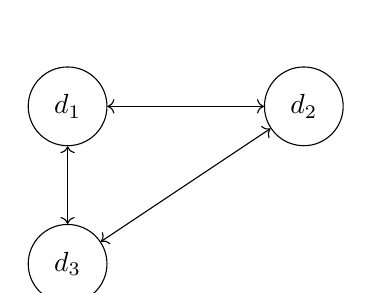
\begin{tikzpicture}[node distance=3cm]
    \node[circle, draw, minimum size=1cm] (d1) {$d_1$};
    \node[circle, draw, minimum size=1cm, right of=d1] (d2) {$d_2$};
    \node[circle, draw, minimum size=1cm, below of=d1, yshift=1cm] (d3) {$d_3$};
    
    \draw[<->] (d1) -- (d2);
    \draw[<->] (d1) -- (d3);
    \draw[<->] (d2) -- (d3);
\end{tikzpicture}
\end{center}

\subsubsection{Initial State Configuration}

The initial state of our example problem is:

\begin{itemize}
    \item \textbf{At dock $d_1$}: Pile $p_1$ contains two containers: $c_1$ (on top) and $c_2$ (below)
    \item \textbf{At dock $d_2$}: 
    \begin{itemize}
        \item Pile $p_2$ contains one container: $c_3$
        \item Pile $p_3$ is empty
    \end{itemize}
    \item \textbf{At dock $d_3$}: Pile $p_4$ is empty
\end{itemize}

\subsection{Formal Representation}

\subsubsection{Objects and Types}

The domain contains objects of different \textbf{sorts} (types). Each object is represented by a constant symbol with an associated type:

\textbf{Docks}: 
\[
\text{Docks} = \{d_1, d_2, d_3\}
\]
where each $d_i$ is a constant symbol of sort $\texttt{Dock}$.

\textbf{Containers}:
\[
\text{Containers} = \{c_1, c_2, c_3\}
\]
where each $c_i$ is a constant symbol of sort $\texttt{Container}$.

\textbf{Robots}:
\[
\text{Robots} = \{r_1, r_2\}
\]
where each $r_i$ is a constant symbol of sort $\texttt{Robot}$.

\textbf{Piles}:
\[
\text{Piles} = \{p_1, p_2, p_3, p_4\}
\]
where each $p_i$ is a constant symbol of sort $\texttt{Pile}$.

The complete set of objects is:
\[
\text{Objects} = \text{Docks} \cup \text{Piles} \cup \text{Containers} \cup \text{Robots}
\]

\subsubsection{Static Relations}

Some relations in the domain are \textbf{static}—they do not change during plan execution. These can be specified once and remain constant throughout.

\textbf{Adjacency relation}: Specifies which docks are directly connected, allowing robots to travel between them.

\[
\texttt{adjacent} = \{(d_1, d_3), (d_3, d_1), (d_2, d_3), (d_3, d_2), (d_1, d_2), (d_2, d_1)\}
\]

This relation is symmetric: if dock $d_i$ is adjacent to dock $d_j$, then $d_j$ is adjacent to $d_i$.

\textbf{Pile-Dock association}: Each pile is permanently located at a specific dock.

\[
\begin{array}{l}
\texttt{at}(p_1, d_1) \\
\texttt{at}(p_2, d_2) \\
\texttt{at}(p_3, d_2) \\
\texttt{at}(p_4, d_3)
\end{array}
\]

\subsubsection{Rigid Relations}

The adjacency relation is defined over $\texttt{Docks} \times \texttt{Docks}$. This is called a \textbf{rigid relation} (also known as a \textbf{static relation})—it does not change during plan execution. Actions cannot modify the physical layout of the docks or their connectivity.

Rigid relations are important because:
\begin{itemize}
    \item They reduce the state space by factoring out unchanging aspects
    \item They can be checked once at planning time rather than during execution
    \item They simplify action preconditions by providing fixed background knowledge
\end{itemize}

\subsection{State Representation in DWR}

\subsubsection{What is a State?}

A \textbf{state} is an assignment of values to propositional variables. More precisely, a state can be represented in two equivalent ways:

\begin{enumerate}
    \item \textbf{First-order ground atoms}: Predicates where all arguments are constants (no variables)
    \item \textbf{First-order ground terms}: Terms where all arguments are constants
\end{enumerate}

\textbf{Important restriction}: We only allow \textbf{flat expressions}, meaning expressions with depth 1 (no nesting).

\begin{example}[Forbidden Nesting]
Consider the predicate $\texttt{loc}(x, y)$ meaning "the location of $x$ is $y$". We do \textbf{not} allow nested expressions such as:
\[
\texttt{loc}(r_1, \texttt{loc}(r_2))
\]
This would represent "the location of $r_1$ is the location of $r_2$", which violates the flatness constraint.
\end{example}

All atoms and terms must be flat—arguments of predicates and functions must be constants, not complex expressions.

\subsubsection{State as Truth Assignment}

A state assigns truth values to ground atoms. Consider describing the initial state $s_0$ of our DWR example:

\[
\begin{array}{l}
\texttt{loc}(r_1, d_1) \\
\texttt{pos}(p_1, d_1) \\
\texttt{pos}(c_2, p_1)
\end{array}
\]

These atoms being listed in the state means they are \textbf{implicitly assigned true}:

\[
\begin{array}{lcl}
\texttt{loc}(r_1, d_1) & \leftarrow & \text{true} \\
\texttt{pos}(p_1, d_1) & \leftarrow & \text{true} \\
\texttt{pos}(c_2, p_1) & \leftarrow & \text{true}
\end{array}
\]

Atoms not mentioned in the state are assumed false (closed-world assumption).

\subsection{Two Representation Formalisms}

There are two common approaches to representing planning problems, differing in how they encode state information.

\subsubsection{Classical (Propositional) Representation}

In the \textbf{classical representation}, states are represented using only \textbf{Boolean assignments} to propositional atoms. Each possible fact about the world is represented as a Boolean variable.

\textbf{Example atoms}:
\begin{itemize}
    \item $\texttt{loc}(r_1, d_1)$: Robot $r_1$ is at dock $d_1$ (true/false)
    \item $\texttt{pos}(c_2, p_1)$: Container $c_2$ is at pile $p_1$ (true/false)
    \item $\texttt{empty}(r_1)$: Robot $r_1$ is not carrying anything (true/false)
\end{itemize}

\textbf{Characteristics}:
\begin{itemize}
    \item Simple and uniform representation
    \item Direct correspondence to propositional logic
    \item Easy to encode as SAT problems
    \item May require many atoms for complex domains
\end{itemize}

\subsubsection{State Variable Representation}

The \textbf{state variable representation} uses a slightly different syntax based on \textbf{function symbols}. Instead of Boolean atoms, we use variables that can take on different values from a finite domain.

\textbf{Example}:
\[
\texttt{loc}(r_1) = d_1
\]

This means "the location of robot $r_1$ is $d_1$". Here, $\texttt{loc}(r_1)$ is a \textbf{state variable} (a function that returns a value), and $d_1$ is its current value.

\textbf{Comparison with classical representation}:

\begin{center}
\begin{tabular}{|l|l|}
\hline
\textbf{Classical} & \textbf{State Variable} \\
\hline
$\texttt{loc}(r_1, d_1) = \text{true}$ & $\texttt{loc}(r_1) = d_1$ \\
$\texttt{loc}(r_1, d_2) = \text{false}$ & \\
$\texttt{loc}(r_1, d_3) = \text{false}$ & \\
\hline
\end{tabular}
\end{center}

\textbf{Advantages of state variables}:
\begin{itemize}
    \item More compact: one variable instead of multiple Boolean atoms
    \item Explicitly represents mutual exclusion (robot can only be at one location)
    \item Natural for domains with multi-valued attributes
    \item Reduces the number of variables in SAT encodings
\end{itemize}

\textbf{Relationship}:
The two representations are \textbf{equivalent in expressive power}. Any problem representable in one formalism can be translated to the other. The choice depends on:
\begin{itemize}
    \item The planning algorithm being used
    \item The structure of the domain
    \item Efficiency considerations for the specific problem
\end{itemize}

\subsubsection{Example: Complete State Representation}

Let us represent the complete initial state $s_0$ of our DWR example in both formalisms.

\textbf{Classical representation} (partial):
\[
\begin{array}{l}
\texttt{loc}(r_1, d_1) = \text{true} \\
\texttt{loc}(r_2, d_2) = \text{true} \\
\texttt{pos}(c_1, p_1) = \text{true} \\
\texttt{pos}(c_2, p_1) = \text{true} \\
\texttt{pos}(c_3, p_2) = \text{true} \\
\texttt{on}(c_1, c_2) = \text{true} \\
\texttt{empty}(r_1) = \text{true} \\
\texttt{empty}(r_2) = \text{true} \\
\texttt{top}(c_1, p_1) = \text{true} \\
\texttt{top}(c_3, p_2) = \text{true}
\end{array}
\]

\textbf{State variable representation}:
\[
\begin{array}{l}
\texttt{loc}(r_1) = d_1 \\
\texttt{loc}(r_2) = d_2 \\
\texttt{pos}(c_1) = p_1 \\
\texttt{pos}(c_2) = p_1 \\
\texttt{pos}(c_3) = p_2 \\
\texttt{on}(c_1) = c_2 \\
\texttt{loaded}(r_1) = \text{nil} \\
\texttt{loaded}(r_2) = \text{nil} \\
\texttt{top}(p_1) = c_1 \\
\texttt{top}(p_2) = c_3
\end{array}
\]

Both representations capture the same information but organize it differently. The state variable representation is more compact and explicitly enforces constraints (e.g., a robot can only be at one location).

\subsection{Key Insight: States as Boolean Assignments}

The fundamental insight is that regardless of the representation formalism chosen:

\begin{center}
\fbox{\textbf{A state is fundamentally a Boolean assignment}}
\end{center}

Whether we use propositional atoms or state variables, we are ultimately assigning truth values (or equivalently, values from finite domains) to a set of variables.

\section{Action Schemas in DWR}

\subsection{Structure of Action Schemas}

An \textbf{action schema} $\alpha$ is a template for generating ground actions. It consists of:

\begin{tcolorbox}[colback=green!5!white,colframe=green!75!black,title=\textbf{Action Schema Components}]
\begin{definition}[Action Schema]
An action schema $\alpha$ has the following components:
\begin{itemize}
    \item \textbf{Name and parameters}: $\alpha: \texttt{name}(z_1, z_2, \dots, z_k)$ where $z_i$ are typed parameters
    \item \textbf{Preconditions}: $\text{Pre}(\alpha) = \{p_1, p_2, \dots, p_n\}$ where each $p_i$ is a literal
    \item \textbf{Effects}: $\text{Eff}(\alpha) = \{q_1, q_2, \dots, q_m\}$ where each $q_i$ is a literal
    \item \textbf{Cost}: $c(\alpha) \in \mathbb{N}_0$ (typically a non-negative integer)
\end{itemize}
\end{definition}
\end{tcolorbox}

\textbf{Important constraint}: The parameters $z_i$ of $\alpha$ can appear in the precondition literals $p_j$ and effect literals $q_j$. The arguments in these literals can be either:
\begin{itemize}
    \item \textbf{Constants}: Specific objects from the domain
    \item \textbf{Parameters}: Variables that will be instantiated
\end{itemize}

No arbitrary free variables are allowed—all variables must be parameters of the action schema.

\begin{tcolorbox}[colback=green!5!white,colframe=green!75!black,title=\textbf{Ground Action}]
\begin{definition}[Ground Action]
A \textbf{ground action} $a$ is obtained by substituting all parameters $z_i$ in action schema $\alpha$ with specific constants from the domain. The action $a$ is an \textbf{instance} of $\alpha$.
\end{definition}
\end{tcolorbox}

\subsection{Example: Take/Load Action}

Consider the action of a robot taking a container from a pile. We define the action schema:

\[
\alpha: \texttt{take}(r, c, c', p, d)
\]

\textbf{Parameters}:
\begin{itemize}
    \item $r$: robot (type $\texttt{Robot}$)
    \item $c$: container to take (type $\texttt{Container}$)
    \item $c'$: container below $c$ (type $\texttt{Container} \cup \{\texttt{nil}\}$)
    \item $p$: pile (type $\texttt{Pile}$)
    \item $d$: dock (type $\texttt{Dock}$)
\end{itemize}

\subsubsection{Correcting Static Relations}

Before defining the preconditions, we note that there are \textbf{two rigid (static) relations} in the DWR domain:

\begin{enumerate}
    \item $\texttt{adjacent}: \texttt{Docks} \times \texttt{Docks}$ — specifies which docks are connected
    \item $\texttt{at}: \texttt{Piles} \times \texttt{Docks}$ — specifies which pile is located at which dock
\end{enumerate}

Both relations are rigid because the physical layout of the port does not change during plan execution.

\subsubsection{Preconditions}

For the \texttt{take} action to be executable, the following conditions must hold:

\[
\text{Pre}(\texttt{take}(r, c, c', p, d)) = \left\{
\begin{array}{l}
\texttt{loc}(r) = d \\
\texttt{at}(p, d) \\
\texttt{pos}(c) = p \\
\texttt{on}(c) = c' \\
\texttt{top}(p) = c \\
\texttt{cargo}(r) = \texttt{nil}
\end{array}
\right\}
\]

\textbf{Interpretation}:
\begin{itemize}
    \item The robot $r$ is at dock $d$
    \item The pile $p$ is located at dock $d$ (static relation)
    \item Container $c$ is positioned at pile $p$
    \item Container $c$ is on top of container $c'$ (or $c'$ is $\texttt{nil}$ if $c$ is at the bottom)
    \item Container $c$ is the top container of pile $p$
    \item The robot $r$ is not carrying anything
\end{itemize}

\subsubsection{Effects}

When the \texttt{take} action is executed, the following changes occur:

\[
\text{Eff}(\texttt{take}(r, c, c', p, d)) = \left\{
\begin{array}{l}
\texttt{cargo}(r) = c \\
\texttt{top}(p) = c' \\
\texttt{pos}(c) = r
\end{array}
\right\}
\]

\textbf{Interpretation}:
\begin{itemize}
    \item The robot $r$ is now carrying container $c$
    \item The top of pile $p$ is now $c'$ (the container that was below $c$)
    \item The position of container $c$ is now the robot $r$
\end{itemize}

\subsection{Action Applicability}

\begin{tcolorbox}[colback=purple!5!white,colframe=purple!75!black,title=\textbf{Action Applicability}]
\begin{definition}[Action Applicability]
A ground action $a$ is \textbf{applicable} (or \textbf{executable}) in state $s$ if all preconditions of $a$ are satisfied in $s$:
\[
a \text{ applicable in } s \quad \Leftrightarrow \quad s \models \text{Pre}(a)
\]
\end{definition}
\end{tcolorbox}

\subsubsection{Examples}

Consider two ground actions:

\textbf{Example 1}: $a_1 = \texttt{take}(r_1, c_1, c_2, p_1, d_1)$

In the initial state $s_0$ where:
\begin{itemize}
    \item $\texttt{loc}(r_1) = d_1$
    \item $\texttt{at}(p_1, d_1)$
    \item $\texttt{pos}(c_1) = p_1$
    \item $\texttt{on}(c_1) = c_2$
    \item $\texttt{top}(p_1) = c_1$
    \item $\texttt{cargo}(r_1) = \texttt{nil}$
\end{itemize}

All preconditions are satisfied, so $a_1$ is \textbf{executable/applicable} in $s_0$.

\textbf{Example 2}: $a_2 = \texttt{take}(r_2, c_3, \texttt{nil}, p_4, d_3)$

This action requires:
\begin{itemize}
    \item $\texttt{loc}(r_2) = d_3$
    \item $\texttt{at}(p_4, d_3)$
    \item $\texttt{pos}(c_3) = p_4$
    \item $\texttt{top}(p_4) = c_3$
\end{itemize}

However, in $s_0$, we have $\texttt{pos}(c_3) = p_2$ (not $p_4$) and $\texttt{loc}(r_2) = d_2$ (not $d_3$). Therefore, $a_2$ is \textbf{not executable/not applicable} in $s_0$.

\section{State Transition Function}

\subsection{Formal Definition}

The \textbf{state transition function} $\gamma$ defines how actions transform states:

\[
\gamma: \text{State} \times \text{Action} \rightarrow \text{State}
\]

where $\gamma(s, a)$ computes the successor state obtained by executing ground action $a$ in state $s$.

\subsection{Computing the Successor State}

Given a state $s$ and a ground action $a$ (which is a ground instance of an action schema $\alpha$), the successor state $\gamma(s, a) = s'$ is defined if and only if:

\begin{enumerate}
    \item $s \models p$ for all $p \in \text{Pre}(a)$ (all preconditions are satisfied)
    \item $s'$ is consistent (the resulting state contains no contradictions)
\end{enumerate}

The successor state $s'$ is computed as:

\[
s' = \{q \mid q \in \text{Eff}(a)\} \cup \{q \mid s \models q, \, \neg q \notin \text{Eff}(a), \, q \notin \text{Eff}(a)\}
\]

\textbf{Interpretation}: The new state consists of:
\begin{itemize}
    \item All literals in the effects of $a$
    \item All literals from $s$ that are not affected by $a$ (neither the literal nor its negation appears in the effects)
\end{itemize}

\subsection{Goal States}

While the initial state is a specific assignment, goals are typically specified more flexibly.

\begin{tcolorbox}[colback=cyan!5!white,colframe=cyan!75!black,title=\textbf{Goal Specification}]
\begin{definition}[Goal Formula]
A \textbf{goal formula} $G$ is a conjunction of literals specifying desired properties of goal states.
\end{definition}

\begin{definition}[Goal States]
The set of \textbf{goal states} is:
\[
S_g = \{ s \mid s \models G \}
\]
That is, all state assignments that satisfy the goal formula $G$.
\end{definition}
\end{tcolorbox}



\subsection{Comparing Representations: Simplified DWR Example}

Let us compare the classical and state variable representations using a simplified version of the DWR domain with three action schemas.

\subsubsection{Classical Representation}

In the classical representation, we use propositional atoms to represent facts:

\textbf{Action 1}: $\texttt{take}(r, c, l)$ — robot $r$ takes container $c$ at location $l$

\[
\begin{array}{ll}
\text{Pre:} & \texttt{loc}(r, l) \land \texttt{pos}(c, l) \land \neg \texttt{loaded}(r) \\
\text{Eff:} & \texttt{pos}(c, r) \land \neg \texttt{pos}(c, l) \land \texttt{loaded}(r)
\end{array}
\]

\textbf{Action 2}: $\texttt{move}(r, l, m)$ — robot $r$ moves from location $l$ to location $m$

\[
\begin{array}{ll}
\text{Pre:} & \texttt{loc}(r, l) \\
\text{Eff:} & \texttt{loc}(r, m) \land \neg \texttt{loc}(r, l)
\end{array}
\]

\textbf{Action 3}: $\texttt{put}(r, c, l)$ — robot $r$ puts down container $c$ at location $l$

\[
\begin{array}{ll}
\text{Pre:} & \texttt{loc}(r, l) \land \texttt{pos}(c, r) \\
\text{Eff:} & \texttt{pos}(c, l) \land \neg \texttt{pos}(c, r) \land \neg \texttt{loaded}(r)
\end{array}
\]

\subsubsection{State Variable Representation}

In the state variable representation, we use functional notation with assignments:

\textbf{Action 1}: $\texttt{take}(r, c, l)$

\[
\begin{array}{ll}
\text{Pre:} & \texttt{loc}(r) = l \land \texttt{pos}(c) = l \land \neg \texttt{loaded}(r) \\
\text{Eff:} & \texttt{pos}(c) \leftarrow r \land \texttt{loaded}(r)
\end{array}
\]

\textbf{Action 2}: $\texttt{move}(r, l, m)$

\[
\begin{array}{ll}
\text{Pre:} & \texttt{loc}(r) = l \\
\text{Eff:} & \texttt{loc}(r) \leftarrow m
\end{array}
\]

\textbf{Action 3}: $\texttt{put}(r, c, l)$

\[
\begin{array}{ll}
\text{Pre:} & \texttt{loc}(r) = l \land \texttt{pos}(c) = r \\
\text{Eff:} & \texttt{pos}(c) \leftarrow l \land \neg \texttt{loaded}(r)
\end{array}
\]

\subsubsection{Key Differences}

\begin{itemize}
    \item \textbf{Classical}: Requires explicit deletion of old values (e.g., $\neg \texttt{loc}(r, l)$ when moving)
    \item \textbf{State Variable}: Implicit deletion through reassignment (e.g., $\texttt{loc}(r) \leftarrow m$ automatically removes the old location)
    \item \textbf{Compactness}: State variables are more concise for multi-valued attributes
\end{itemize}

\section{Planning as Satisfiability (SAT)}

\subsection{Recap: Core Concepts}

Before introducing the SAT encoding, let us recap the fundamental concepts:

\begin{itemize}
    \item \textbf{State}: A Boolean assignment to propositional (ground) literals
    \item \textbf{Action}: Characterized by:
    \begin{itemize}
        \item \textbf{Preconditions}: A set (or conjunction) of literals
        \item \textbf{Effects}: A set (or conjunction) of literals
    \end{itemize}
\end{itemize}

\subsection{Temporal Instantiation of Variables}

To encode planning problems as SAT, we introduce a temporal dimension to our propositional variables.

\begin{tcolorbox}[colback=blue!5!white,colframe=blue!75!black,title=\textbf{Temporal Instantiation}]
\begin{definition}[Temporal Instantiation]
Let $X$ be the set of propositional variables describing the domain. The \textbf{temporal instantiation} of $X$ at time $t$ is:
\[
X@t = \{x@t \mid x \in X\} \quad \text{for } t \geq 0
\]
where $x@t$ is a propositional variable representing the truth value of $x$ at time step $t$.
\end{definition}
\end{tcolorbox}

\textbf{Intuition}: Since a plan is a sequence of actions $(a_0, a_1, a_2, \dots, a_{n-1})$ of length $n$, we need to track the truth value of each proposition at each time step from $0$ to $n$.

\subsection{The Bounded Planning Problem}

\begin{tcolorbox}[colback=orange!10!white,colframe=orange!75!black,title=\textbf{Bounded Planning Problem}]
\begin{definition}[Bounded Planning Problem]
Given a planning problem $P = \langle \Sigma, I, G \rangle$, the \textbf{bounded planning problem} asks:

\textit{Does there exist a plan solving $P$ with length exactly $n$?}
\end{definition}
\end{tcolorbox}

This is a decision problem parameterized by the plan length $n$.

\subsection{SAT Encoding}

The bounded planning problem can be encoded as a propositional satisfiability problem.

\begin{tcolorbox}[colback=red!5!white,colframe=red!75!black,title=\textbf{Planning as SAT}]
\begin{theorem}[Planning as SAT]
For a planning problem $P$ and bound $n$, there exists a propositional formula $\Phi_n$ such that:
\[
\Phi_n \text{ is satisfiable} \quad \Leftrightarrow \quad \text{there exists a plan of length } n \text{ for } P
\]
\end{theorem}
\end{tcolorbox}

The formula $\Phi_n$ encodes:
\begin{enumerate}
    \item \textbf{Initial state}: $I@0$ (the initial state holds at time 0)
    \item \textbf{Goal state}: $G@n$ (the goal holds at time $n$)
    \item \textbf{Action preconditions and effects}: For each time step $t \in \{0, 1, \dots, n-1\}$, exactly one action is executed and its effects are correctly applied
    \item \textbf{Frame axioms}: Variables not affected by actions remain unchanged
\end{enumerate}

\subsection{Solving Planning via Iterative Deepening}

Since we don't know the optimal plan length in advance, we use \textbf{iterative deepening}:

\begin{tcolorbox}[colback=yellow!10!white,colframe=yellow!75!black,title=\textbf{Iterative Deepening SAT Planning}]
\begin{algorithm}[H]
\caption{Planning via SAT with Iterative Deepening}
\begin{algorithmic}[1]
\STATE $n \leftarrow 1$
\WHILE{true}
    \STATE Construct formula $\Phi_n$
    \IF{$\Phi_n$ is satisfiable}
        \STATE Extract plan from satisfying assignment
        \RETURN plan
    \ENDIF
    \STATE $n \leftarrow n + 1$
\ENDWHILE
\end{algorithmic}
\end{algorithm}
\end{tcolorbox}

\textbf{Process}:
\begin{enumerate}
    \item Try $n = 1$: Check if $\Phi_1$ is satisfiable
    \item If not, try $n = 2$: Check if $\Phi_2$ is satisfiable
    \item If not, try $n = 3$: Check if $\Phi_3$ is satisfiable
    \item Continue until a satisfiable formula is found
\end{enumerate}

\textbf{Advantages}:
\begin{itemize}
    \item Finds shortest plans (optimal in number of steps)
    \item Leverages highly optimized SAT solvers
    \item Scales well for many planning domains
\end{itemize}

\textbf{Challenges}:
\begin{itemize}
    \item Formula size grows with $n$
    \item May need to try many values of $n$ before finding a solution
    \item Encoding frame axioms can be expensive
\end{itemize}



\newpage

\part{SAT Solvers and Planning}

\section{The Boolean Satisfiability Problem}

\subsection{Definition and Scope}

The \textbf{Boolean Satisfiability Problem (SAT)} is one of the most fundamental problems in computer science and forms the foundation for many automated reasoning techniques, including planning.

\begin{tcolorbox}[colback=blue!5!white,colframe=blue!75!black,title=\textbf{SAT Problem}]
\begin{definition}[SAT Problem]
The SAT problem asks: Given a propositional formula, does there exist an interpretation (truth assignment) that makes the formula true?

Formally, given a set of clauses $S$ in propositional logic, determine whether $S$ is satisfiable.
\end{definition}
\end{tcolorbox}

\subsection{Propositional Logic Basics}

To understand SAT, we must first establish the basic elements of propositional logic:

\begin{itemize}
    \item \textbf{Propositional variables}: Let $X$ be a finite set of propositional variables, where each variable can assume one of two values: \texttt{true} (1) or \texttt{false} (0)
    
    \item \textbf{Atom (Atomic formula)}: A single propositional variable $x \in X$
    
    \item \textbf{Literal}: Either an atom $x$ or its negation $\neg x$
    
    \item \textbf{Clause}: A disjunction of literals: $L_1 \lor L_2 \lor \cdots \lor L_n$ where each $L_i$ is a literal
\end{itemize}

\subsection{Interpretations and Truth Assignments}

\begin{tcolorbox}[colback=green!5!white,colframe=green!75!black,title=\textbf{Interpretation}]
\begin{definition}[Interpretation]
An \textbf{interpretation} (or \textbf{truth assignment}) is a function:
\[
v: X \rightarrow \{0, 1\}
\]
that assigns a Boolean value to each propositional variable.
\end{definition}
\end{tcolorbox}

\textbf{Number of interpretations}: If $|X| = n$ (i.e., we have $n$ propositional variables), then there are exactly $2^n$ possible interpretations.

\subsubsection{Satisfiability of Clauses}

\begin{tcolorbox}[colback=purple!5!white,colframe=purple!75!black,title=\textbf{Satisfaction}]
\begin{definition}[Clause Satisfaction]
A clause $C = L_1 \lor L_2 \lor \cdots \lor L_n$ is \textbf{satisfied} by an interpretation $v$ if there exists at least one literal $L_i$ such that $v(L_i) = \text{true}$ for some $i \in \{1, 2, \dots, n\}$.

We write: $v \models C$
\end{definition}

\begin{definition}[Formula Satisfaction]
A set of clauses $S = \{C_1, C_2, \dots, C_m\}$ is \textbf{satisfiable} if there exists an interpretation $v$ that satisfies all clauses in $S$:
\[
v \models S \quad \Leftrightarrow \quad v \models C_i \text{ for all } i \in \{1, 2, \dots, m\}
\]
\end{definition}
\end{tcolorbox}

\subsection{SAT Decision Procedure}

The SAT problem can be viewed as a decision procedure with the following input-output specification:

\[
\boxed{
\begin{array}{ccc}
S \text{ (set of clauses)} & \xrightarrow{\text{SAT Solver}} & 
\begin{cases}
\text{\textbf{YES (Satisfiable)}} \\
\exists v: v \models S \\
\\
\text{\textbf{NO (Unsatisfiable)}} \\
\text{Proof: } S \vdash \Box
\end{cases}
\end{array}
}
\]

\textbf{Output cases}:
\begin{enumerate}
    \item \textbf{YES (Satisfiable)}: There exists an interpretation $v$ such that $v \models S$. The SAT solver typically returns this satisfying assignment.
    
    \item \textbf{NO (Unsatisfiable)}: No interpretation satisfies $S$. The solver may provide a proof of unsatisfiability, showing that $S$ derives a contradiction (denoted $S \vdash \Box$, where $\Box$ represents the empty clause).
\end{enumerate}

\subsection{The Empty Clause}

\begin{tcolorbox}[colback=red!5!white,colframe=red!75!black,title=\textbf{Empty Clause}]
\begin{definition}[Empty Clause]
The \textbf{empty clause}, denoted $\Box$ (or $\square$), is a clause with no literals. It is \textbf{false in all interpretations} and therefore represents a contradiction.
\end{definition}
\end{tcolorbox}

\textbf{Significance}: If a SAT solver derives the empty clause from the input formula $S$, this constitutes a proof that $S$ is unsatisfiable, since deriving a contradiction means no interpretation can satisfy all clauses.




\section{Planning Problem Formalization}

We formalized the planning problem with:
\[
P = \langle \Sigma, s_0, S_g \rangle
\]
where $\Sigma = \langle S, A, \gamma \rangle$.

\begin{itemize}
    \item $s_0$ is the initial state
    \item $S_g$ is the set of goal states: $S_g = \{s \mid s \models G\}$
    \item $G$ is the goal formula (a conjunction of atoms)
\end{itemize}

\subsection{States as Interpretations}

States correspond to interpretations in propositional logic:

\begin{itemize}
    \item $\texttt{at}(r_1, l_1)$: ground positive literal
    \item $\neg \texttt{loaded}(r_1)$: ground negative literal
\end{itemize}

\textbf{Abstraction}: From ground first-order literals to propositional literals. With finitely many ground atoms (literals) in the planning problem, we obtain finitely many variables $|X| = n$.

\section{Bounded Planning Problem}

\begin{definition}[Bounded Planning Problem]
Does there exist a plan $\pi$ that solves planning problem $P$ and has length $k$ (i.e., $|\pi| = k$, where $\pi$ is a sequence of $k$ actions)?
\end{definition}

\subsection{Iterative Deepening on Plan Length}

We use iterative deepening to find the shortest plan by increasing the bound $k$:

\[
\boxed{
\begin{array}{c}
P \xrightarrow{\text{translation}} \Phi \xrightarrow{\text{SAT}} 
\begin{cases}
\text{\textbf{YES}}: \text{interpretation } v \models \Phi \\
\text{encodes plan } \pi \text{ of length } k \\
\text{\textbf{NO}}: \text{no plan of length } k \text{ solves } P
\end{cases}
\end{array}
}
\]

The process iterates: $k := k + 1$ until a solution is found.

\textbf{Key insight}: The SAT encoding $\Phi$ includes:
\begin{itemize}
    \item Initial state constraints at time 0
    \item Goal constraints at time $k$
    \item Action preconditions and effects for each time step
    \item Frame axioms ensuring persistence of unchanged literals
\end{itemize}





\subsection{Temporal Encoding of Literals}

A key aspect of the SAT encoding for planning is the \textbf{temporal instantiation} of literals. Since a plan of length $k$ requires tracking state changes over time, each literal is indexed by time steps.

\begin{itemize}
    \item \textbf{Plan length $k$} means we have $0 \leq i \leq k-1$ time steps (transitions)
    \item Each literal $f$ becomes $f@t$ where $t$ ranges from $0$ to $k$
    \item State $i$ is the state after executing $i$ actions (before the $i$-th action)
\end{itemize}

\subsubsection{Example: Temporal Instantiation}

Consider the literal $\texttt{at}(r_1, l_1)$ ("robot $r_1$ is at location $l_1$"):

\[
\texttt{at}(r_1, l_1) \quad \xrightarrow{\text{temporal encoding}} \quad \texttt{at}(r_1, l_1, i)
\]

Similarly, the negative literal $\neg \texttt{loaded}(r_1)$ becomes $\neg \texttt{loaded}(r_1, i)$, meaning "robot $r_1$ is not loaded at stage $i$".

\begin{tcolorbox}[colback=cyan!5!white,colframe=cyan!75!black,title=\textbf{State Transition}]
\begin{definition}[State Transition]
Step $i$ (where $0 \leq i \leq k-1$) takes us from state $i$ to state $i+1$ by executing one action.
\end{definition}
\end{tcolorbox}

\subsection{Encoding the Initial State}

The initial state $s_0$ is encoded as a conjunction of constraints at time $t = 0$:

\[
\Phi_{s_0} = \bigwedge_{f \in s_0} f@0 \quad \land \quad \bigwedge_{f \notin s_0} \neg f@0
\]

Where $f$ represents ground literals.

\subsubsection{From Literals to Propositional Variables}

Each temporally indexed literal corresponds to a propositional variable:

\begin{itemize}
    \item $\texttt{at}(r_1, l_1, 0)$ corresponds to variable $x_{\texttt{at}(r_1, l_1)}@0$
    \item $\neg \texttt{loaded}(r_1, 0)$ corresponds to $\neg x_{\texttt{loaded}(r_1)}@0$
\end{itemize}

\subsubsection{Example: Complete Initial State Encoding}

Consider an initial state containing $\texttt{at}(r_1, l_1)$ but not $\texttt{loaded}(r_1)$:

\[
\begin{array}{lcl}
\text{Literals in } s_0: & \texttt{at}(r_1, l_1) & \land \neg \texttt{loaded}(r_1) \land \cdots \\
\text{Temporal encoding:} & \texttt{at}(r_1, l_1, 0) & \land \neg \texttt{loaded}(r_1, 0) \land \cdots \\
\text{SAT variables:} & x_{\texttt{at}(r_1, l_1)}@0 & \land \neg x_{\texttt{loaded}(r_1)}@0 \land \cdots
\end{array}
\]

For literals not in the initial state (e.g., $\texttt{at}(r_1, l_2)$, $\texttt{at}(r_1, l_3)$), these are assigned false:

\[
\neg \texttt{at}(r_1, l_2, 0), \quad \neg \texttt{at}(r_1, l_3, 0)
\]

\textbf{Alternative notation}: The initial state encoding can also be written using set notation:
\[
\Phi_{s_0} = \bigwedge_{x \in S_0^+} x_0 \land \bigwedge_{x \in S_0^-} \neg x_0
\]
where $S_0^+$ is the set of positive literals in $s_0$ and $S_0^-$ is the set of negative literals in $s_0$.

\subsection{Encoding the Goal States}

The goal conditions must be satisfied at the final time step $k$.

\begin{tcolorbox}[colback=green!5!white,colframe=green!75!black,title=\textbf{Goal Encoding}]
\begin{definition}[Goal Encoding]
The goal states are encoded at time $k$ as:
\[
\Phi_G = \bigwedge_{x \in G^+} x_k \land \bigwedge_{x \in G^-} \neg x_k
\]
where $G^+$ is the set of positive literals in the goal $G$ and $G^-$ is the set of negative literals in $G$.
\end{definition}
\end{tcolorbox}

\textbf{Interpretation}: This formula ensures that all positive goal conditions are true and all negative goal conditions are false in the final state after executing $k$ actions.

\subsection{Encoding Actions}

The planning problem is defined as $\Sigma = \langle S, A, \gamma \rangle$, where $A$ is the set of all ground instances of the action schemas.

\subsubsection{Action Preconditions}

For each action $a \in A$ at each time step $i$ (where $0 \leq i \leq k-1$), we encode the constraint that if the action is executed, its preconditions must hold:

\begin{tcolorbox}[colback=yellow!10!white,colframe=yellow!75!black,title=\textbf{Action Precondition Encoding}]
\begin{definition}[Action Precondition Encoding]
\[
\forall a \in A, \forall i \in \{0, \dots, k-1\}: \quad a_i \rightarrow \bigwedge_{p \in \text{prec}(a)} p_i
\]
where $\text{prec}(a)$ denotes the set of preconditions of action $a$.
\end{definition}
\end{tcolorbox}

\textbf{Interpretation}: This formula states that if action $a$ is executed at time $i$, then all of its preconditions must be satisfied at time $i$. The implication can be rewritten in CNF as:
\[
\neg a_i \lor \bigwedge_{p \in \text{prec}(a)} p_i
\]

\subsubsection{Mutual Exclusion of Actions}

At each time step, at most one action can be executed. This constraint is encoded as follows:

\begin{tcolorbox}[colback=orange!10!white,colframe=orange!75!black,title=\textbf{Action Mutual Exclusion}]
\begin{definition}[Action Mutual Exclusion]
For all pairs of distinct actions \( (a, b) \in A \times A \) where \( a \neq b \), and for all time steps \( i \) where \( 0 \leq i \leq k-1 \):
\[
\neg a_i \lor \neg b_i
\]
\end{definition}
\end{tcolorbox}

This formula ensures that actions \( a \) and \( b \) cannot both be executed at the same time step \( i \).

\textbf{Equivalent formulations}:
\begin{itemize}
    \item \( a_i \rightarrow \neg b_i \): If action \( a \) is executed at time \( i \), then action \( b \) is not executed
    \item \( b_i \rightarrow \neg a_i \): If action \( b \) is executed at time \( i \), then action \( a \) is not executed
\end{itemize}

\subsection{Complete SAT Encoding}

The complete SAT encoding \( \Phi \) for a bounded planning problem with plan length \( k \) is the conjunction of the following sets of propositional formulas:

\[
\Phi = \Phi_{s_0} \land \Phi_G \land \Phi_{\text{actions}} \land \Phi_{\text{mutex}} \land \Phi_{\text{frame}}
\]

where:
\begin{itemize}
    \item \( \Phi_{s_0} \): Initial state constraints
    \item \( \Phi_G \): Goal state constraints
    \item \( \Phi_{\text{actions}} \): Action precondition and effect constraints
    \item \( \Phi_{\text{mutex}} \): Mutual exclusion constraints between actions
    \item \( \Phi_{\text{frame}} \): Frame axioms (persistence of unchanged literals)
\end{itemize}

\subsection{Plan Extraction from SAT Model}

Once the SAT solver returns a satisfying assignment, we can extract the corresponding plan.

\begin{tcolorbox}[colback=teal!10!white,colframe=teal!75!black,title=\textbf{Plan Extraction}]
\begin{definition}[Plan Extraction]
Let \( v \) be a satisfying interpretation (model) returned by the SAT solver, represented as a set of literals. The plan \( \pi \) is extracted as follows:

\[
\pi = \langle a_0, a_1, \dots, a_{k-1} \rangle
\]

where \( a_i \) is the unique action such that \( v \models a_i \) (i.e., \( a_i \) is assigned \texttt{true} in the model \( v \)) for each time step \( i \in \{0, 1, \dots, k-1\} \).
\end{definition}
\end{tcolorbox}

\textbf{Extraction procedure}:
\begin{enumerate}
    \item Filter the model \( v \) to obtain only the action literals: \( \{a_i \mid a \in A, 0 \leq i \leq k-1, v \models a_i\} \)
    \item For each time step \( i \), identify the action \( a \) such that \( a_i \) is true in \( v \)
    \item Construct the sequence \( \pi = \langle a_0, a_1, \dots, a_{k-1} \rangle \)
\end{enumerate}

\begin{remark}
Due to the mutual exclusion constraints, at most one action is true at each time step. If no action is true at some time step \( i \), this corresponds to a "no-op" (no operation) action.
\end{remark}



\newpage

\part{SAT Encoding Examples}

\section{Detailed SAT Encoding Example}

\subsection{Simple Robot Navigation Domain}

To illustrate the complete SAT encoding process, we present a simple example with a single robot and two locations.

\begin{example}[Robot Navigation]
Consider a minimal planning domain with the following components:

\textbf{Objects}:
\begin{itemize}
    \item One robot: $r_1$
    \item Two locations: $l_1$, $l_2$
\end{itemize}

\textbf{Action schema}: $\texttt{move}(r, l, l')$

\[
\begin{array}{ll}
\text{Parameters:} & r \text{ (robot)}, l \text{ (source location)}, l' \text{ (destination location)} \\
\text{Precondition:} & \texttt{at}(r, l) \\
\text{Effect:} & \texttt{at}(r, l') \land \neg \texttt{at}(r, l)
\end{array}
\]
\end{example}

\subsubsection{Ground Actions}

With one robot and two locations, we obtain two ground actions:

\begin{enumerate}
    \item $a_1 = \texttt{move}(r_1, l_1, l_2)$: Move robot $r_1$ from location $l_1$ to location $l_2$
    \item $a_2 = \texttt{move}(r_1, l_2, l_1)$: Move robot $r_1$ from location $l_2$ to location $l_1$
\end{enumerate}

\subsubsection{Problem Instance}

\textbf{Initial state} (at time step $t = 0$):
\[
s_0 = \{\texttt{at}(r_1, l_1)\}
\]

The robot starts at location $l_1$. This is encoded temporally as:
\[
\texttt{at}(r_1, l_1)@0
\]

\textbf{Goal state} (at time step $t = 1$):
\[
G = \{\texttt{at}(r_1, l_2)\}
\]

The goal is for the robot to be at location $l_2$ after one action. This is encoded as:
\[
\texttt{at}(r_1, l_2)@1
\]

\subsection{Complete SAT Encoding}

For this problem with plan length $k = 1$, we construct the following propositional formulas:

\subsubsection{Initial State Constraints}

\[
\Phi_{s_0} = \texttt{at}(r_1, l_1)@0 \land \neg \texttt{at}(r_1, l_2)@0
\]

\subsubsection{Goal State Constraints}

\[
\Phi_G = \texttt{at}(r_1, l_2)@1
\]

\subsubsection{Action Preconditions and Effects}

For action $a_1 = \texttt{move}(r_1, l_1, l_2)$ at time step $0$:
\[
\texttt{move}(r_1, l_1, l_2)@0 \rightarrow \big(\texttt{at}(r_1, l_1)@0 \land \texttt{at}(r_1, l_2)@1 \land \neg \texttt{at}(r_1, l_1)@1\big)
\]

For action $a_2 = \texttt{move}(r_1, l_2, l_1)$ at time step $0$:
\[
\texttt{move}(r_1, l_2, l_1)@0 \rightarrow \big(\texttt{at}(r_1, l_2)@0 \land \texttt{at}(r_1, l_1)@1 \land \neg \texttt{at}(r_1, l_2)@1\big)
\]

\subsubsection{Explanatory Frame Axioms}

The \textbf{explanatory frame axioms} (also called \textbf{explanation axioms}) state that if a literal changes its truth value between time steps, then some action causing that change must have been executed.

\textbf{If $\texttt{at}(r_1, l_1)$ becomes false}:
\[
\texttt{at}(r_1, l_1)@0 \land \neg \texttt{at}(r_1, l_1)@1 \rightarrow \texttt{move}(r_1, l_1, l_2)@0
\]

\textbf{If $\texttt{at}(r_1, l_2)$ becomes false}:
\[
\texttt{at}(r_1, l_2)@0 \land \neg \texttt{at}(r_1, l_2)@1 \rightarrow \texttt{move}(r_1, l_2, l_1)@0
\]

\textbf{If $\texttt{at}(r_1, l_1)$ becomes true}:
\[
\neg \texttt{at}(r_1, l_1)@0 \land \texttt{at}(r_1, l_1)@1 \rightarrow \texttt{move}(r_1, l_2, l_1)@0
\]

\textbf{If $\texttt{at}(r_1, l_2)$ becomes true}:
\[
\neg \texttt{at}(r_1, l_2)@0 \land \texttt{at}(r_1, l_2)@1 \rightarrow \texttt{move}(r_1, l_1, l_2)@0
\]

\subsection{Solution Extraction}

Given the constraints, the SAT solver will find a satisfying assignment that includes:

\[
\texttt{move}(r_1, l_1, l_2)@0 = \text{true}
\]

The extracted plan is:
\[
\pi = \langle \texttt{move}(r_1, l_1, l_2) \rangle
\]

This plan has length $1$ and achieves the goal of moving the robot from $l_1$ to $l_2$.

\section{Conversion to Conjunctive Normal Form}

\subsection{CNF Definition and Structure}

To use a SAT solver, we must convert all formulas to \textbf{Conjunctive Normal Form (CNF)}.

\begin{tcolorbox}[colback=blue!5!white,colframe=blue!75!black,title=\textbf{Conjunctive Normal Form (CNF)}]
\begin{definition}[Clause]
A \textbf{clause} is a disjunction of literals: $L_1 \lor L_2 \lor \cdots \lor L_k$ where each $L_i$ is a literal (an atom or its negation).
\end{definition}

\begin{definition}[Conjunctive Normal Form (CNF)]
A formula is in \textbf{Conjunctive Normal Form} if it is a conjunction of clauses:
\[
\text{CNF} = (L_1^1 \lor L_2^1 \lor \cdots \lor L_k^1) \land (L_1^2 \lor L_2^2 \lor \cdots \lor L_k^2) \land \cdots \land (L_1^m \lor L_2^m \lor \cdots \lor L_k^m)
\]
\end{definition}
\end{tcolorbox}

A set of clauses is logically equivalent to a conjunction of those clauses, which is precisely the CNF representation required by SAT solvers.

\subsection{Standard CNF Transformation}

The standard transformation to CNF involves applying logical equivalences to eliminate implications and biconditionals, push negations inward, and distribute disjunctions over conjunctions.

\subsubsection{Logical Equivalences}

The following logical equivalences are used in the transformation:

\textbf{Biconditional elimination}:
\[
F \leftrightarrow G \equiv (F \rightarrow G) \land (G \rightarrow F)
\]

\textbf{Implication elimination}:
\[
F \rightarrow G \equiv \neg F \lor G
\]

\textbf{De Morgan's laws}:
\[
\begin{array}{lcl}
\neg(F \lor G) &\equiv& \neg F \land \neg G \\
\neg(F \land G) &\equiv& \neg F \lor \neg G
\end{array}
\]

\subsubsection{Negation Normal Form (NNF)}

After applying the above equivalences, we obtain a formula in \textbf{Negation Normal Form (NNF)}, where negations appear only directly in front of atoms (not in front of complex formulas).

\subsubsection{Distribution to Obtain CNF}

To convert from NNF to CNF, we apply the \textbf{distributive law}:

\[
F \lor (G \land H) \equiv (F \lor G) \land (F \lor H)
\]

This distributes disjunctions over conjunctions, eventually producing a conjunction of disjunctions (CNF).

\subsection{The Exponential Blowup Problem}

\textbf{Critical issue}: The standard CNF transformation can cause a \textbf{combinatorial explosion} in formula size.

\begin{tcolorbox}[colback=red!5!white,colframe=red!75!black,title=\textbf{Exponential Blowup Problem}]
\begin{observation}[Exponential Blowup]
In the worst case, the standard transformation into CNF produces a formula whose size is \textbf{exponential} in the size of the original formula: $O(2^n)$ where $n$ is the size of the input formula.
\end{observation}
\end{tcolorbox}

This exponential blowup makes the standard transformation \textbf{impractical} for large planning problems, as the resulting CNF formula becomes too large to handle efficiently.

\subsection{Equisatisfiable CNF (ECNF)}

To avoid the exponential blowup, we use a different approach that produces an \textbf{Equisatisfiable CNF (ECNF)}.

\begin{tcolorbox}[colback=green!5!white,colframe=green!75!black,title=\textbf{Equisatisfiable CNF (ECNF)}]
\begin{definition}[Equisatisfiable CNF]
An \textbf{Equisatisfiable CNF (ECNF)} is a CNF formula that is not logically equivalent to the original formula, but is \textbf{equisatisfiable}—it has the same satisfiability status:
\begin{itemize}
    \item The original formula is satisfiable if and only if the ECNF is satisfiable
    \item The ECNF may contain additional auxiliary variables not present in the original formula
\end{itemize}
\end{definition}
\end{tcolorbox}

\subsubsection{Tseitin Encoding}

The standard technique for producing ECNF is the \textbf{Tseitin encoding} (also called \textbf{Tseitin transformation}), named after Grigori Tseitin.

\textbf{Key idea}: Introduce auxiliary variables to represent subformulas, avoiding the need for distribution.

\begin{tcolorbox}[colback=purple!5!white,colframe=purple!75!black,title=\textbf{Tseitin Encoding Complexity}]
\begin{theorem}[Tseitin Encoding Complexity]
The Tseitin encoding produces an ECNF formula whose size is \textbf{linear} in the size of the original formula: $O(n)$ where $n$ is the size of the input formula.
\end{theorem}
\end{tcolorbox}

\textbf{Advantages of ECNF}:
\begin{itemize}
    \item \textbf{Linear size}: Avoids exponential blowup
    \item \textbf{Preserves satisfiability}: The ECNF is satisfiable if and only if the original formula is satisfiable
    \item \textbf{Efficient encoding}: Can be computed in polynomial time
    \item \textbf{Practical for planning}: Makes SAT-based planning feasible for large problems
\end{itemize}

\textbf{Trade-off}:
\begin{itemize}
    \item The ECNF introduces additional variables (one for each subformula)
    \item The ECNF is not logically equivalent to the original formula (only equisatisfiable)
    \item However, the satisfying assignments to the original variables correspond to solutions of the original formula
\end{itemize}

\subsection{Tseitin Encoding: Formal Construction}

The Tseitin encoding is based on two key functions that work together to produce the ECNF.

\subsubsection{The Representative Function}

\begin{tcolorbox}[colback=cyan!5!white,colframe=cyan!75!black,title=\textbf{Representative Function}]
\begin{definition}[Representative Function]
Let $\text{PL}$ denote the language of propositional formulas over a set of propositional variables $X$, and let $V$ be a set of fresh (new) propositional variables. The \textbf{representative function} is defined as:
\[
\text{Rep}: \text{PL} \rightarrow V \cup \{\bot, \top\}
\]
\end{definition}
\end{tcolorbox}

The function $\text{Rep}$ assigns to each formula a representative variable (or constant). It is defined inductively:

\textbf{Base case} (atomic formulas):
\[
\begin{array}{lcl}
\text{Rep}(x) &=& x \quad \text{for all } x \in X \\
\text{Rep}(\bot) &=& \bot \\
\text{Rep}(\top) &=& \top
\end{array}
\]

\textbf{Inductive case} (complex formulas):
\[
\text{Rep}(F) = v_F
\]
where $F \in \text{PL}$ is a non-atomic formula (i.e., $F$ is neither a propositional variable nor $\bot$ nor $\top$), and $v_F \in V$ is a fresh propositional variable uniquely associated with $F$.

\textbf{Intuition}: Each complex subformula is represented by a new auxiliary variable. This avoids the need to duplicate subformulas during the transformation.

\subsubsection{The Encoding Function}

\begin{tcolorbox}[colback=cyan!5!white,colframe=cyan!75!black,title=\textbf{Encoding Function}]
\begin{definition}[Encoding Function]
The \textbf{encoding function} is defined as:
\[
\text{En}: \text{PL} \rightarrow \text{PL}
\]
\[
\text{En}(F) = F \leftrightarrow \text{Rep}(F)
\]
\end{definition}
\end{tcolorbox}

The encoding function creates a biconditional formula stating that formula $F$ is logically equivalent to its representative.

\textbf{Interpretation}: $\text{En}(F)$ encodes the constraint that the auxiliary variable $\text{Rep}(F)$ must have the same truth value as the formula $F$ itself.

\subsubsection{Complete ECNF Construction}

\begin{tcolorbox}[colback=orange!10!white,colframe=orange!75!black,title=\textbf{ECNF via Tseitin Encoding}]
\begin{definition}[ECNF via Tseitin Encoding]
Given an input formula $F$, let $S_F$ denote the set of all subformulas of $F$ (including $F$ itself). The \textbf{Equisatisfiable CNF} of $F$ is:
\[
\text{ECNF}(F) = \text{Rep}(F) \land \bigwedge_{G \in S_F} \text{En}(G)
\]
\end{definition}
\end{tcolorbox}

\textbf{Components}:
\begin{itemize}
    \item $\text{Rep}(F)$: The representative variable for the entire formula (must be true)
    \item $\bigwedge_{G \in S_F} \text{En}(G)$: Conjunction of encoding constraints for all subformulas
\end{itemize}

\textbf{Why "Equisatisfiable"?}

The transformation from $F$ to $\text{ECNF}(F)$ does \textbf{not} preserve logical equivalence, but it \textbf{does} preserve satisfiability:

\begin{tcolorbox}[colback=yellow!10!white,colframe=yellow!75!black,title=\textbf{Equisatisfiability Theorem}]
\begin{theorem}[Equisatisfiability]
Formula $F$ is satisfiable if and only if $\text{ECNF}(F)$ is satisfiable.
\end{theorem}
\end{tcolorbox}

\begin{proof}[Proof sketch]
\textbf{Forward direction} ($F$ satisfiable $\Rightarrow$ $\text{ECNF}(F)$ satisfiable):
If $F$ is satisfiable, we can extend the satisfying assignment to include the auxiliary variables by setting each $v_G = \text{value}(G)$ under the original assignment. This satisfies all encoding constraints.

\textbf{Backward direction} ($\text{ECNF}(F)$ satisfiable $\Rightarrow$ $F$ satisfiable):
If $\text{ECNF}(F)$ is satisfiable, the encoding constraints ensure that $\text{Rep}(F)$ has the same truth value as $F$. Since $\text{Rep}(F)$ must be true (it appears as a conjunct), $F$ must also be true under the restriction of the assignment to the original variables.
\end{proof}

\textbf{Key insight}: The ECNF introduces auxiliary variables but maintains the same satisfiability status as the original formula, while keeping the formula size linear.

\subsection{Example: Equisatisfiability vs. Logical Equivalence}

To illustrate the difference between equisatisfiability and logical equivalence, consider a concrete example.

\begin{example}[Tseitin Encoding of Disjunction]
Consider the formula:
\[
F = A \lor (B \land C)
\]
where $A$, $B$, and $C$ are propositional variables.

Using the standard CNF transformation (distribution), we would obtain:
\[
F_{\text{CNF}} = (A \lor B) \land (A \lor C)
\]

This is \textbf{logically equivalent} to $F$, but for larger formulas, this approach leads to exponential blowup.
\end{example}

\subsubsection{Tseitin Encoding Approach}

Instead, we apply the Tseitin encoding by introducing an auxiliary variable $v$ to represent the subformula $B \land C$:

\textbf{Step 1}: Define the encoding constraint:
\[
v \leftrightarrow (B \land C)
\]

\textbf{Step 2}: Replace the subformula in the original formula:
\[
A \lor v
\]

\textbf{Step 3}: Convert the biconditional to CNF. The biconditional $v \leftrightarrow (B \land C)$ expands to:
\[
(v \rightarrow (B \land C)) \land ((B \land C) \rightarrow v)
\]

Converting each implication:
\begin{align*}
v \rightarrow (B \land C) &\equiv \neg v \lor (B \land C) \equiv (\neg v \lor B) \land (\neg v \lor C) \\
(B \land C) \rightarrow v &\equiv \neg(B \land C) \lor v \equiv \neg B \lor \neg C \lor v
\end{align*}

\textbf{Final ECNF}: The complete set of clauses is:
\[
S = \{(A \lor v), \, (\neg v \lor B), \, (\neg v \lor C), \, (\neg B \lor \neg C \lor v)\}
\]

Numbering the clauses:
\begin{align*}
(1) &\quad A \lor v \\
(2) &\quad \neg v \lor B \\
(3) &\quad \neg v \lor C \\
(4) &\quad \neg B \lor \neg C \lor v
\end{align*}

\subsubsection{Demonstrating Equisatisfiability}

Consider the interpretation:
\[
I = \{A \mapsto \text{true}, \, B \mapsto \text{false}, \, C \mapsto \text{false}\}
\]

\textbf{Evaluating $F$ under $I$}:
\[
F = A \lor (B \land C) = \text{true} \lor (\text{false} \land \text{false}) = \text{true} \lor \text{false} = \text{true}
\]

Therefore, $I \models F$ (interpretation $I$ satisfies $F$).

\textbf{Evaluating $S$ under $I$}:

We need to extend $I$ to assign a value to the auxiliary variable $v$. Let's first try without extending:

\begin{itemize}
    \item Clause (1): $A \lor v = \text{true} \lor v = \text{true}$ \quad (satisfied regardless of $v$)
    \item Clause (2): $\neg v \lor B = \neg v \lor \text{false} = \neg v$ \quad (satisfied only if $v = \text{false}$)
    \item Clause (3): $\neg v \lor C = \neg v \lor \text{false} = \neg v$ \quad (satisfied only if $v = \text{false}$)
    \item Clause (4): $\neg B \lor \neg C \lor v = \text{true} \lor \text{true} \lor v = \text{true}$ \quad (satisfied regardless of $v$)
\end{itemize}

For $I$ to satisfy $S$, we must set $v = \text{false}$ (to satisfy clauses (2) and (3)). With this extension:
\[
I' = \{A \mapsto \text{true}, \, B \mapsto \text{false}, \, C \mapsto \text{false}, \, v \mapsto \text{false}\}
\]

Now $I' \models S$ (all clauses are satisfied).

\begin{tcolorbox}[colback=teal!10!white,colframe=teal!75!black,title=\textbf{Equisatisfiability vs Logical Equivalence}]
\begin{observation}[Not Logically Equivalent]
The original interpretation $I$ (without the auxiliary variable) satisfies $F$ but does \textbf{not} satisfy all clauses in $S$ unless extended with the appropriate value for $v$. This demonstrates that $F$ and $S$ are \textbf{not logically equivalent}.

However, $F$ is satisfiable if and only if $S$ is satisfiable (by appropriately choosing the value of $v$). Therefore, $F$ and $S$ are \textbf{equisatisfiable}.
\end{observation}
\end{tcolorbox}

\textbf{Conclusion}: The Tseitin encoding produces a formula that is equisatisfiable with the original but not logically equivalent. This is acceptable for SAT-based planning because we only care about whether a solution exists, not about preserving all logical properties.

\subsection{Detailed Definition of the Encoding Function}

We now provide the complete formal definition of the encoding function $\text{En}$ for all cases.

\begin{definition}[Encoding Function - Complete Definition]
The encoding function $\text{En}: \text{PL} \rightarrow \text{PL}$ is defined inductively as follows:

\textbf{Base cases} (atomic formulas):
\[
\begin{array}{lcl}
\text{En}(\bot) &=& \top \\
\text{En}(\top) &=& \top \\
\text{En}(x) &=& \top \quad \text{for all } x \in X
\end{array}
\]

\textbf{Inductive case for negation}:
\begin{align*}
\text{En}(\neg F) &= \text{let } v = \text{Rep}(\neg F) \text{ in } v \leftrightarrow \neg \text{Rep}(F) \\
&= (v \rightarrow \neg \text{Rep}(F)) \land (\neg \text{Rep}(F) \rightarrow v) \\
&= (\neg v \lor \neg \text{Rep}(F)) \land (\text{Rep}(F) \lor v)
\end{align*}

\textbf{Inductive case for binary connectives}:

For all binary connectives $\circ \in \{\land, \lor, \rightarrow, \leftrightarrow\}$:
\[
\text{En}(F_1 \circ F_2) = \text{let } v = \text{Rep}(F_1 \circ F_2) \text{ in } v \leftrightarrow (\text{Rep}(F_1) \circ \text{Rep}(F_2))
\]
\end{definition}

\subsubsection{Example: Conjunction Encoding}

\begin{example}[Encoding Conjunction]
Consider the encoding of $F_1 \land F_2$:

\begin{align*}
\text{En}(F_1 \land F_2) &= \text{let } v = \text{Rep}(F_1 \land F_2) \text{ in } v \leftrightarrow (\text{Rep}(F_1) \land \text{Rep}(F_2)) \\
&= (v \rightarrow (\text{Rep}(F_1) \land \text{Rep}(F_2))) \land ((\text{Rep}(F_1) \land \text{Rep}(F_2)) \rightarrow v) \\
&= (\neg v \lor (\text{Rep}(F_1) \land \text{Rep}(F_2))) \land ((\text{Rep}(F_1) \land \text{Rep}(F_2)) \lor v)
\end{align*}

Distributing to obtain CNF:
\[
(\neg v \lor \text{Rep}(F_1)) \land (\neg v \lor \text{Rep}(F_2)) \land (\text{Rep}(F_1) \lor v) \land (\text{Rep}(F_2) \lor v)
\]

This produces \textbf{4 clauses} in CNF.
\end{example}

\subsection{Complexity Analysis of Tseitin Encoding}

We now analyze the size of the resulting ECNF formula to prove linear complexity.

\begin{tcolorbox}[colback=purple!5!white,colframe=purple!75!black,title=\textbf{Linear Size of ECNF}]
\begin{theorem}[Linear Size of ECNF]
Let $F$ be a propositional formula with size $|F| = n$. The Tseitin encoding produces an ECNF formula:
\[
F' = \text{Rep}(F) \land \bigwedge_{G \in S_F} \text{En}(G)
\]
where $S_F$ is the set of all subformulas of $F$ (including $F$ itself). The size of $F'$ is $|F'| = O(n)$.
\end{theorem}
\end{tcolorbox}

\subsubsection{Worst Case Analysis: Biconditional}

The worst case for the encoding function occurs with the biconditional connective. Let us analyze:

\begin{example}[Biconditional Encoding - Complete Derivation]
We show the complete step-by-step conversion of the biconditional encoding to CNF:

\textbf{Step 1}: Start with the encoding
\begin{align*}
\text{En}(F_1 \leftrightarrow F_2) &= \text{let } v = \text{Rep}(F_1 \leftrightarrow F_2) \text{ in } v \leftrightarrow (\text{Rep}(F_1) \leftrightarrow \text{Rep}(F_2))
\end{align*}

\textbf{Step 2}: Expand the inner biconditional
\begin{align*}
&= v \leftrightarrow [(\text{Rep}(F_1) \rightarrow \text{Rep}(F_2)) \land (\text{Rep}(F_2) \rightarrow \text{Rep}(F_1))]
\end{align*}

\textbf{Step 3}: Expand the outer biconditional
\begin{align*}
&= \big(v \rightarrow [(\text{Rep}(F_1) \rightarrow \text{Rep}(F_2)) \land (\text{Rep}(F_2) \rightarrow \text{Rep}(F_1))]\big) \\
&\quad \land \big([(\text{Rep}(F_1) \rightarrow \text{Rep}(F_2)) \land (\text{Rep}(F_2) \rightarrow \text{Rep}(F_1))] \rightarrow v\big)
\end{align*}

\textbf{Step 4}: Convert implications to disjunctions
\begin{align*}
&= \big(\neg v \lor [(\text{Rep}(F_1) \rightarrow \text{Rep}(F_2)) \land (\text{Rep}(F_2) \rightarrow \text{Rep}(F_1))]\big) \\
&\quad \land \big(\neg[(\text{Rep}(F_1) \rightarrow \text{Rep}(F_2)) \land (\text{Rep}(F_2) \rightarrow \text{Rep}(F_1))] \lor v\big)
\end{align*}

\textbf{Step 5}: Expand inner implications
\begin{align*}
&= \big(\neg v \lor [(\neg \text{Rep}(F_1) \lor \text{Rep}(F_2)) \land (\neg \text{Rep}(F_2) \lor \text{Rep}(F_1))]\big) \\
&\quad \land \big(\neg[(\neg \text{Rep}(F_1) \lor \text{Rep}(F_2)) \land (\neg \text{Rep}(F_2) \lor \text{Rep}(F_1))] \lor v\big)
\end{align*}

\textbf{Step 6}: Distribute $\neg v$ over the conjunction (first part)
\begin{align*}
&= (\neg v \lor \neg \text{Rep}(F_1) \lor \text{Rep}(F_2)) \land (\neg v \lor \neg \text{Rep}(F_2) \lor \text{Rep}(F_1))
\end{align*}

\textbf{Step 7}: Apply De Morgan's law to the second part
\begin{align*}
&\quad \land \big(\neg(\neg \text{Rep}(F_1) \lor \text{Rep}(F_2)) \lor \neg(\neg \text{Rep}(F_2) \lor \text{Rep}(F_1)) \lor v\big)
\end{align*}

\textbf{Step 8}: Apply De Morgan's law again
\begin{align*}
&\quad \land \big((\text{Rep}(F_1) \land \neg \text{Rep}(F_2)) \lor (\text{Rep}(F_2) \land \neg \text{Rep}(F_1)) \lor v\big)
\end{align*}

\textbf{Step 9}: Distribute disjunction over conjunction
\begin{align*}
&\quad \land (\text{Rep}(F_1) \lor \text{Rep}(F_2) \lor v) \land (\text{Rep}(F_1) \lor \neg \text{Rep}(F_1) \lor v) \\
&\quad \land (\neg \text{Rep}(F_2) \lor \text{Rep}(F_2) \lor v) \land (\neg \text{Rep}(F_2) \lor \neg \text{Rep}(F_1) \lor v)
\end{align*}

\textbf{Step 10}: Simplify (remove tautologies)

The clauses $(\text{Rep}(F_1) \lor \neg \text{Rep}(F_1) \lor v)$ and $(\neg \text{Rep}(F_2) \lor \text{Rep}(F_2) \lor v)$ are tautologies and can be removed.

\textbf{Final CNF}: The encoding produces the following clauses:
\begin{align*}
&(\neg v \lor \neg \text{Rep}(F_1) \lor \text{Rep}(F_2)) \\
&(\neg v \lor \neg \text{Rep}(F_2) \lor \text{Rep}(F_1)) \\
&(\text{Rep}(F_1) \lor \text{Rep}(F_2) \lor v) \\
&(\neg \text{Rep}(F_2) \lor \neg \text{Rep}(F_1) \lor v)
\end{align*}

This produces \textbf{4 clauses} after simplification (or up to 8 clauses before removing tautologies).
\end{example}

\begin{proof}[Proof of Linear Complexity]
\textbf{Key observations}:
\begin{enumerate}
    \item The number of subformulas $|S_F|$ is at most $n$ (the size of $F$)
    \item Each subformula $G \in S_F$ contributes at most a constant number of clauses (at most 8 for biconditional)
    \item Therefore, the total number of clauses is at most $8n$
    \item Each clause has at most 3 literals
    \item Total size: $|F'| \leq 8n \times 3 = 24n = O(n)$
\end{enumerate}

More precisely, we can bound the size as $|F'| = O(30n + 2)$, which is still linear in $n$.
\end{proof}

\textbf{Conclusion}: The Tseitin encoding achieves linear size $O(n)$ instead of the exponential size $O(2^n)$ of the standard CNF transformation, making it practical for large planning problems.


\newpage
\part{SAT Decision Procedures}

\section{Decision Procedures for Satisfiability}

We now present a \textbf{decision procedure} for determining the satisfiability of a set of clauses. This procedure is fundamental to understanding how SAT solvers work and forms the algorithmic foundation for planning via SAT encoding.

\begin{tcolorbox}[colback=blue!5!white,colframe=blue!75!black,title=\textbf{SAT Decision Problem}]
\begin{definition}[SAT Decision Problem]
Given a set of clauses $S$ over a set of Boolean variables $X$, determine whether there exists a model (satisfying assignment) $v: X \rightarrow \{\text{true}, \text{false}\}$ such that $v \models S$.
\end{definition}
\end{tcolorbox}

\subsection{Relation to Constraint Solving}

The SAT problem is closely related to \textbf{Constraint Solving Problems (CSP)} with Boolean variables. It represents one of the most fundamental problems in algorithmic theory and was the first problem proven to be \textbf{NP-complete}.

\[
\boxed{
\begin{array}{ccc}
S \text{ (set of clauses)} & \xrightarrow{\text{SAT Decision Procedure}} &
\begin{cases}
\text{\textbf{YES (Satisfiable)}} \\
\exists v: v \models S \\
\\
\text{\textbf{NO (Unsatisfiable)}} \\
\text{with proof: } S \vdash \Box
\end{cases}
\end{array}
}
\]

\section{State Representation and Search Modes}

\subsection{Trail-Based State Representation}

The state of the SAT decision procedure is represented using a \textbf{trail} of literals, which maintains the current partial assignment of truth values to variables.

\begin{tcolorbox}[colback=green!5!white,colframe=green!75!black,title=\textbf{Trail Representation}]
\begin{definition}[Trail]
A \textbf{trail} $\varGamma$ is a sequence of literals representing the current partial assignment in the search process. The empty trail is denoted $\varepsilon$.
\end{definition}

\begin{definition}[Search State]
A search state is represented as a pair $\langle S, \varGamma \rangle$ where:
\begin{itemize}
    \item $S$ is the current set of clauses
    \item $\varGamma$ is the current trail (partial assignment)
\end{itemize}
\end{definition}
\end{tcolorbox}

\subsection{Literal Status in Trails}

Given a trail $\varGamma$ and a literal $L$, the status of $L$ is determined as follows:

\begin{itemize}
    \item $L$ is \textbf{true} if $L \in \varGamma$
    \item $L$ is \textbf{false} if $\neg L \in \varGamma$
    \item $L$ is \textbf{undefined} if neither $L$ nor $\neg L$ appears in $\varGamma$
\end{itemize}

\section{Transition Rules}

The SAT decision procedure operates as a \textbf{transition system} with specific rules that transform the search state. There are two main types of transitions:

\subsection{Decision Rule}

The \textbf{decision rule} extends the trail by choosing an undefined literal and adding it to the current assignment.

\begin{tcolorbox}[colback=purple!5!white,colframe=purple!75!black,title=\textbf{Decision Rule}]
\begin{definition}[Decision Transition]
\[
\langle S \parallel \varGamma \rangle \rightarrow \langle S \parallel \varGamma, L \rangle
\]
where the decision is applicable if:
\begin{itemize}
    \item $L \notin \varGamma$ (literal not already assigned)
    \item $\neg L \notin \varGamma$ (negation not already assigned)
\end{itemize}
\end{definition}
\end{tcolorbox}

The decision rule represents a \textbf{choice point} in the search process where the algorithm guesses a truth value for an undefined variable.

\subsection{Propagation Rule}

The \textbf{propagation rule} (also called \textbf{unit propagation}) adds literals that are logically implied by the current assignment.

\begin{tcolorbox}[colback=orange!10!white,colframe=orange!75!black,title=\textbf{Propagation Rule}]
\begin{definition}[Propagation Transition]
\[
\langle S \parallel \varGamma \rangle \rightarrow \langle S \parallel \varGamma, L \rangle
\]
where the propagation is applicable if there exists a clause $C = L_1 \lor L_2 \lor \cdots \lor L_{k-1} \lor L_k \in S$ such that:
\begin{itemize}
    \item $D = L_1 \lor L_2 \lor \cdots \lor L_{k-1}$
    \item $\varGamma \models \neg D$ (all literals in $D$ are false under current assignment)
    \item $L = L_k$ (the remaining literal becomes implied)
    \item $L \notin \varGamma$ and $\neg L \notin \varGamma$
\end{itemize}
\end{definition}
\end{tcolorbox}

\subsubsection{Justification for Implied Literals}

When a literal $L_k$ is propagated with justification clause $C$, it means:

\begin{itemize}
    \item The clause $C = L_1 \lor L_2 \lor \cdots \lor L_{k-1} \lor L_k$ must be satisfied
    \item All other literals $L_1, L_2, \dots, L_{k-1}$ are currently false under $\varGamma$
    \item Therefore, $L_k$ must be true to satisfy the clause
\end{itemize}

This is called the \textbf{justification} for the propagation: the clause $C$ forces $L_k$ to be true.

\subsubsection{Logical Foundation of Propagation}

The propagation rule is based on the following logical principle:

If we have a clause $D \lor L$ where $D = L_1 \lor L_2 \lor \cdots \lor L_{k-1}$, and we know that $\neg D$ (i.e., $\neg L_1 \land \neg L_2 \land \cdots \land \neg L_{k-1}$), then:

\[
\neg D \models L
\]

Because if all the alternative literals are false, the remaining literal must be true to satisfy the disjunction.

\section{Solution States}

The search process terminates when it reaches specific terminal states:

\begin{tcolorbox}[colback=cyan!5!white,colframe=cyan!75!black,title=\textbf{Solution States}]
\begin{itemize}
    \item \textbf{Success}: The state $\langle S, \varGamma \rangle$ where all clauses in $S$ are satisfied by the assignment represented by $\varGamma$
    \item \textbf{Failure}: The state where a conflict is detected (e.g., the empty clause $\Box$ is derived)
\end{itemize}
\end{tcolorbox}

The decision procedure systematically explores the space of possible assignments using these transition rules until it either finds a satisfying assignment or proves that no such assignment exists.

\section{Conflict Analysis and Learning}

When the propagation rule leads to a conflict (derivation of the empty clause $\Box$), the SAT solver enters \textbf{conflict analysis mode} to learn from the conflict and guide future search.

\subsection{Conflict-Solving Mode}

\begin{tcolorbox}[colback=red!5!white,colframe=red!75!black,title=\textbf{Conflict State Representation}]
\begin{definition}[Conflict State]
A state in conflict-solving mode is represented as a triple $\langle S \parallel \varGamma \parallel C \rangle$ where:
\begin{itemize}
    \item $S$ is the current set of clauses
    \item $\varGamma$ is the current trail (partial assignment)
    \item $C$ is the \textbf{conflict clause} that caused the conflict
\end{itemize}
\end{definition}
\end{tcolorbox}

The conflict clause $C$ represents a learned constraint that explains why the current partial assignment leads to a contradiction. This clause can be added to the formula to prevent the same conflict in future search branches.

\subsection{Search Space Complexity}

The SAT decision procedure explores a search space that grows exponentially with the number of variables.

\begin{tcolorbox}[colback=orange!10!white,colframe=orange!75!black,title=\textbf{Search Space Size}]
\begin{definition}[Search Space Complexity]
Given a SAT problem with $n$ Boolean variables, the total number of possible assignments is:
\[
2^n
\]
where each variable can be assigned either true or false.
\end{definition}
\end{tcolorbox}

\subsubsection{Search Tree Structure}

The search process forms a binary tree where each level corresponds to a variable assignment. For two variables $p$ and $Q$, the search space has the following structure:

\begin{itemize}
    \item \textbf{Level 0}: Start state
    \item \textbf{Level 1}: Variable $p$ can be assigned $1$ or $0$
    \item \textbf{Level 2}: For each assignment of $p$, variable $Q$ can be assigned $1$ or $0$
\end{itemize}

This creates four possible complete assignments:
\begin{itemize}
    \item $p=1, Q=1$
    \item $p=1, Q=0$
    \item $p=0, Q=0$
    \item $p=0, Q=1$
\end{itemize}

For $n$ variables, this creates a complete binary tree of depth $n$ with $2^n$ leaves, representing all possible assignments.

\section{Backtracking Mechanism}

When a conflict is detected or a dead-end is reached, the solver uses \textbf{backtracking} to explore alternative assignments.

\subsection{Backtracking Rule}

\begin{tcolorbox}[colback=purple!5!white,colframe=purple!75!black,title=\textbf{Backtracking Transition}]
\begin{definition}[Backtracking]
\[
\langle S \parallel M \, L^d \, N \parallel C \rangle \rightarrow \langle S \parallel M \, \neg L^d \rangle
\]
where:
\begin{itemize}
    \item $M$ is the sequence of literals before the decision
    \item $L^d$ is the most recent \textbf{decided literal} (marked with $d$)
    \item $N$ is the sequence of literals after the decision
    \item The transition is only applicable if $N$ contains no decided literals
\end{itemize}
\end{definition}
\end{tcolorbox}

Backtracking implements a \textbf{depth-first search strategy} that:
\begin{itemize}
    \item Explores one branch of the search tree completely before trying alternatives
    \item When a conflict occurs, backtracks to the most recent decision point
    \item Flips the decision (from $L^d$ to $\neg L^d$) and continues search from there
\end{itemize}

\subsection{Decision vs. Propagated Literals}

The distinction between decided and propagated literals is crucial for backtracking:

\begin{itemize}
    \item \textbf{Decided literals} ($L^d$): Chosen by the decision rule, can be flipped during backtracking
    \item \textbf{Propagated literals}: Forced by unit propagation, cannot be flipped (would immediately cause conflict)
\end{itemize}

The backtracking rule only flips decided literals, ensuring that propagated assignments remain consistent.

\section{Termination and Results}

The search process terminates when it reaches one of two possible outcomes:

\subsection{Success State}

\begin{tcolorbox}[colback=green!5!white,colframe=green!75!black,title=\textbf{Success Condition}]
\begin{definition}[Satisfiable Instance]
\[
\langle S \parallel \varGamma \rangle \quad \text{returns} \quad (\text{"sat"}, \varGamma)
\]
if and only if $\varGamma \models S$ (i.e., the assignment represented by trail $\varGamma$ satisfies all clauses in $S$).
\end{definition}
\end{tcolorbox}

When a satisfying assignment is found, the solver returns:
\begin{itemize}
    \item Status: \texttt{"sat"} (satisfiable)
    \item Model: The complete assignment $\varGamma$ that satisfies the formula
\end{itemize}

\subsection{Failure State}

\begin{tcolorbox}[colback=red!5!white,colframe=red!75!black,title=\textbf{Failure Condition}]
\begin{definition}[Unsatisfiable Instance]
\[
\langle S \parallel \varGamma \parallel C \rangle \quad \text{returns} \quad \text{"unsat"}
\]
if and only if $\varGamma$ contains no decision literals (i.e., all literals in the trail were propagated, not decided).
\end{definition}
\end{tcolorbox}

When the formula is proven unsatisfiable, the solver returns:
\begin{itemize}
    \item Status: \texttt{"unsat"} (unsatisfiable)
    \item The empty clause $\Box$ serves as a certificate of unsatisfiability
\end{itemize}

This occurs when the solver has exhausted all possible assignments without finding a satisfying one, meaning the formula is logically inconsistent.

\section{Conflict-Driven Clause Learning (CDCL)}

Modern SAT solvers use \textbf{Conflict-Driven Clause Learning (CDCL)}, an advanced technique that combines depth-first search with intelligent learning from conflicts to efficiently solve large satisfiability problems.

\subsection{CDCL Algorithm Overview}

CDCL implements a \textbf{depth-first search strategy} with intelligent backjumping and clause learning:

\begin{tcolorbox}[colback=blue!5!white,colframe=blue!75!black,title=\textbf{CDCL Components}]
\textbf{CDCL} combines several key techniques:
\begin{itemize}
    \item \textbf{Unit propagation}: Efficient inference of forced assignments
    \item \textbf{Conflict analysis}: Learning from failures to guide future search
    \item \textbf{Backjumping}: Intelligent backtracking to earlier decision levels
    \item \textbf{Clause learning}: Adding learned constraints to prevent repeated conflicts
\end{itemize}
\end{tcolorbox}

\subsection{Backjumping: Generalized Backtracking}

Backjumping is a generalization of the basic backtracking mechanism that allows the solver to jump back to earlier decision levels, not just the immediately preceding one.

\begin{tcolorbox}[colback=purple!5!white,colframe=purple!75!black,title=\textbf{Backjumping vs. Backtracking}]
\begin{definition}[Backjumping]
In \textbf{backjumping}, when a conflict occurs, the solver analyzes the conflict clause to determine the earliest decision level that contributed to the conflict. It then jumps back to that level, rather than just the immediately preceding decision.
\end{definition}

\textbf{Advantage}: Backjumping can skip over irrelevant decision levels, significantly reducing the search space compared to basic backtracking.
\end{tcolorbox}

\subsubsection{Conflict Analysis Example}

Consider a conflict clause $C = L_1 \lor \cdots \lor L_k$ where all literals are currently false. The analysis determines:

\begin{itemize}
    \item Why each literal $L_i$ is false in the current trail $\varGamma$
    \item The decision level at which each literal became false
    \item The earliest decision level that contributed to the conflict
\end{itemize}

The solver then backjumps to that earliest relevant decision level, effectively skipping decision levels that did not contribute to the conflict.

\section{Binary Resolution}

The theoretical foundation of conflict analysis in CDCL relies on \textbf{binary resolution}, a fundamental inference rule in propositional logic.

\subsection{Resolution Rule}

\begin{tcolorbox}[colback=green!5!white,colframe=green!75!black,title=\textbf{Binary Resolution}]
\begin{definition}[Binary Resolution]
Given two clauses containing complementary literals:
\[
\frac{C \lor L \quad D \lor \neg L}{(C \lor D)}
\]
where $C$ and $D$ are disjunctions of literals, and $L$ is a literal.
\end{definition}
\end{tcolorbox}

The \textbf{resolvent} $C \lor D$ is logically entailed by the two premises. This rule allows deriving new clauses that preserve satisfiability.

\subsection{Soundness of Resolution}

Binary resolution is \textbf{sound}—the resolvent is logically entailed by the premises.

\begin{tcolorbox}[colback=yellow!10!white,colframe=yellow!75!black,title=\textbf{Soundness Proof}]
\begin{theorem}[Resolution Soundness]
If $\{C \lor L, D \lor \neg L\} \models R$ where $R$ is any formula, then $\{C \lor L, D \lor \neg L\} \models (C \lor D)$.

\begin{proof}
Consider any interpretation $v$:
\begin{itemize}
    \item If $v \models L$, then since $v \models D \lor \neg L$, we must have $v \models D$. Since $v \models C \lor L$, we have $v \models C \lor D$.
    \item If $v \models \neg L$, then since $v \models C \lor L$, we must have $v \models C$. Since $v \models D \lor \neg L$, we have $v \models C \lor D$.
\end{itemize}
In both cases, $v \models C \lor D$, so the resolvent is logically entailed by the premises.
\end{proof}
\end{theorem}
\end{tcolorbox}

\subsection{Application in Conflict Analysis}

In conflict analysis, resolution is used to explain why conflicts occur and to determine which decision levels are responsible:

\begin{itemize}
    \item When a literal $L_k$ in the conflict clause is false due to propagation (not a decision)
    \item The propagation was justified by a clause $D \lor \neg L_k$
    \item By resolving the conflict clause with the justification clause, we can trace back the decision that ultimately caused the conflict
\end{itemize}

\section{Explanation Mechanism}

The explanation mechanism in CDCL traces the implications that led to a conflict, allowing the solver to learn more general constraints.

\begin{tcolorbox}[colback=orange!10!white,colframe=orange!75!black,title=\textbf{Explanation Transition}]
\begin{definition}[Explanation Rule]
\[
\langle S \parallel \varGamma \parallel C \rangle \rightarrow \langle S \parallel \varGamma \parallel C \lor D \rangle
\]
if $\neg L \in \varGamma$ where $\neg L$ was propagated using the clause $D \lor \neg L$.
\end{definition}
\end{tcolorbox}

\subsection{Explanation Process}

The explanation mechanism works as follows:

\begin{enumerate}
    \item Start with a conflict clause $C = L_1 \lor \cdots \lor L_k$
    \item For each literal $L_i$ that is false due to propagation (not a decision):
    \begin{itemize}
        \item Find the justification clause that forced $\neg L_i$ into the trail
        \item Resolve the current conflict clause with the justification clause
        \item Continue until all literals in the conflict clause are explained by decisions
    \end{itemize}
    \item The final resolved clause contains only literals that were decided (not propagated)
    \item This clause can be learned and added to the formula to prevent similar conflicts
\end{enumerate}



\newpage 

\part{SAT-Based Techniques}

\section{Modern SAT Solving}

\subsection{CDCL: An Evolution of DPLL}

CDCL (\textbf{Conflict-Driven Clause Learning}) represents an evolution of the DPLL decision procedure for SAT. While CDCL maintains the same basic decision rule as DPLL, it introduces sophisticated conflict analysis and learning mechanisms that dramatically improve solver efficiency on real-world instances.

\subsubsection{CDCL Transition Rules}

The CDCL procedure employs the following transition rules in search mode:

\begin{tcolorbox}[colback=blue!5!white,colframe=blue!75!black,title=\textbf{Decision Rule}]
\begin{definition}[Decision]
\[
\langle S \parallel \varGamma \rangle \rightarrow \langle S \parallel \varGamma, L^d \rangle
\]
if $L \notin \varGamma$ and $\neg L \notin \varGamma$, where:
\begin{itemize}
    \item $S$ is the set of clauses
    \item $\varGamma$ is the trail (sequence of assigned literals)
    \item $L^d$ is a decision literal (chosen by a heuristic)
\end{itemize}
\end{definition}
\end{tcolorbox}

\begin{tcolorbox}[colback=green!5!white,colframe=green!75!black,title=\textbf{Propagation Rule}]
\begin{definition}[Propagation]
\[
\langle S \parallel \varGamma \rangle \rightarrow \langle S \parallel \varGamma, L_{C\lor L} \rangle
\]
if $C \lor L \in S$, $L \notin \varGamma$, $\neg L \notin \varGamma$, and $\varGamma \models \neg C$, where:
\begin{itemize}
    \item $C$ is a disjunction of literals (all false under the current trail)
    \item $L$ is the unit literal that must be propagated
    \item The subscript $C\lor L$ indicates the justification clause for the propagation
\end{itemize}
\end{definition}
\end{tcolorbox}

\begin{tcolorbox}[colback=green!5!white,colframe=green!75!black,title=\textbf{Success Rule}]
\begin{definition}[Success]
\[
\langle S \parallel \varGamma \rangle \rightarrow \text{"sat"}
\]
if $\varGamma \models S$ (i.e., the trail satisfies all clauses in the set)
\end{definition}
\end{tcolorbox}

\begin{tcolorbox}[colback=red!5!white,colframe=red!75!black,title=\textbf{Conflict Rule}]
\begin{definition}[Conflict]
\[
\langle S \parallel \varGamma \rangle \rightarrow \langle S \parallel \varGamma \parallel C \rangle
\]
if $C \in S$ and $\varGamma \models \neg C$ (i.e., the trail conflicts with clause $C$), where $C$ is the conflict clause that triggers the transition to conflict analysis mode.
\end{definition}
\end{tcolorbox}

These four rules define the behavior of CDCL in \textbf{search mode}, which is identical to the DPLL procedure. The key difference lies in how CDCL handles conflicts through its conflict analysis and learning mechanisms.

\subsection{Decision Levels in CDCL}

The trail $\varGamma$ in CDCL is organized into \textbf{decision levels} that provide structure to the search process:

\begin{itemize}
    \item The trail begins at \textbf{decision level 0} (empty trail)
    \item Each decision literal opens a new decision level
    \item If the maximum decision level in $\varGamma$ is $n$, the next decision opens level $n+1$
    \item All propagations following a decision remain at the same level until the next decision
\end{itemize}

\subsubsection{Trail as a Stack Structure}

The trail can be conceptualized as a \textbf{stack structure}:

\begin{enumerate}
    \item Initially, the stack is empty (decision level 0)
    \item A decision literal is pushed onto the stack, opening a new level
    \item Unit propagations following the decision are pushed onto the stack at the same level
    \item Another decision is made, opening the next level
    \item The process continues with alternating decisions and propagations
    \item During backtracking/backjumping, literals are popped from the stack until reaching the target decision level
\end{enumerate}

This organization enables efficient backjumping by allowing the solver to quickly identify and return to relevant decision levels during conflict analysis.



% --------------------------------------------------
% Example and Conflict Handling
% --------------------------------------------------

\subsection{Illustrative Example}

\begin{tcolorbox}[colback=gray!5!white,colframe=gray!60!black,title=\textbf{Instance}]
$S = \{\, P,\; \neg P \lor Q \lor R,\; T \lor \neg Q,\; \neg R \lor Q \}$
\end{tcolorbox}

\noindent The initial propagation and decision sequence proceeds as follows:
\begin{align*}
\langle S \parallel \epsilon \rangle &\xrightarrow{\text{prop}} \langle S \parallel P_{P} \rangle\\[4pt]
&\xrightarrow{\text{dec}} \langle S \parallel P_{P},\, Q^{d} \rangle\\[4pt]
&\xrightarrow{\text{prop}} \langle S \parallel P_{P},\, Q^{d},\, T_{T \lor \neg Q} \rangle
\end{align*}

\begin{remark}
The trail behaves exactly like a \emph{stack}: each decision opens a new level and subsequent propagations are pushed on top of that level.
\end{remark}

\subsection{Conflict Mode}

When a conflict clause $C$ becomes false under the current trail, the solver enters conflict mode. Two outcomes are possible:
\begin{enumerate}
    \item \textbf{Fail}: The formula is unsatisfiable.
    \item \textbf{Conflict resolution}: The solver analyzes the conflict, learns a new clause, backjumps, and resumes search.
\end{enumerate}

\subsubsection{Fail Rule}

\begin{tcolorbox}[colback=red!5!white,colframe=red!75!black,title=\textbf{Fail Condition}]
\begin{definition}[Unsat at Level 0]
\[
\langle S \parallel \varGamma \parallel C \rangle \; \rightarrow \; \text{"unsat"}
\]
if $\max\operatorname{level}(\varGamma)=0$.
\end{definition}
\end{tcolorbox}

\subsubsection{Explanation Rule}

Assume the conflict clause has the form
\[
C = L_1 \lor L_2 \lor \dots \lor L_{k-1} \lor L_k, \quad \text{all literals false in } \varGamma.
\]
If $\neg L_k$ was propagated by the clause $D \lor \neg L_k$, we resolve $C$ with this justification to obtain a new clause:
\[
C' = L_1 \lor L_2 \lor \dots \lor L_{k-1} \lor D.
\]

\begin{tcolorbox}[colback=orange!10!white,colframe=orange!75!black,title=\textbf{Explanation Transition}]
\begin{definition}
\[
\langle S \parallel \varGamma \parallel C \lor L \rangle \; \rightarrow \; \langle S \parallel \varGamma \parallel C \lor D \rangle
\]
if $\neg L_{D \lor \neg L} \in \varGamma$.
\end{definition}
\end{tcolorbox}

The resolution step is repeated until the resulting clause contains exactly one literal from the current decision level (\emph{1-UIP clause}).

\subsubsection{Learning Rule}

\begin{tcolorbox}[colback=green!5!white,colframe=green!75!black,title=\textbf{Clause Learning}]
\begin{definition}
\[
\langle S \parallel \varGamma \parallel C \rangle \; \rightarrow \; \langle S \cup \{C\} \parallel \varGamma \parallel C \rangle
\]
if $C \notin S$.
\end{definition}
\end{tcolorbox}

The learned clause $C$ prevents the solver from repeating the same conflicting assignment in the future.

\subsubsection{Backjumping Rule}

\begin{tcolorbox}[colback=purple!5!white,colframe=purple!75!black,title=\textbf{Backjumping}]
\begin{definition}
Let $\varGamma = N\,L^d\,M$ where $L^d$ is the most recent decision literal and $C \lor L'$ is the learned clause with $L'$ falsified at level $k<\operatorname{level}(L^d)$. Then
\[
\langle S \parallel N\,L^d\,M \parallel C \lor L' \rangle \; \rightarrow \; \langle S \parallel N \cup \{L'_{C \lor L'}\} \rangle.
\]
\end{definition}
\end{tcolorbox}

Backjumping skips irrelevant decision levels, jumping directly to level $k$, and immediately propagates $L'$ using the learned clause.

% --------------------------------------------------
\vspace{1em}

\subsection{Control Strategy}

The transition rules of CDCL are governed by specific control policies that determine the order in which rules are applied.

\subsubsection{Search Mode Control}

\begin{tcolorbox}[colback=blue!5!white,colframe=blue!75!black,title=\textbf{Search Mode Priority}]
In search mode, \textbf{Propagation} has higher priority than \textbf{Decision}.
\end{tcolorbox}

This ensures that all forced assignments (unit propagations) are made before any heuristic decision is taken, maximizing constraint propagation and reducing the search space.

\subsubsection{Conflict Mode Control}

\begin{tcolorbox}[colback=red!5!white,colframe=red!75!black,title=\textbf{Conflict Mode Sequence}]
The conflict mode rules are applied in the following order:
\[
\text{Explanation}^* \;\rightarrow\; \text{Learning} \;\rightarrow\; \text{Backjumping}
\]
where Explanation$^*$ denotes repeated application of the Explanation rule.
\end{tcolorbox}

\subsection{First Assertion Clause Heuristic}

The \textbf{First Assertion Clause (FAC)} heuristic is a widely used strategy for determining when to stop the explanation process and perform backjumping.

\begin{tcolorbox}[colback=yellow!10!white,colframe=yellow!75!black,title=\textbf{Assertion Clause}]
\begin{definition}[Assertion Clause]
An \textbf{assertion clause} is a conflict clause $C \lor L'$ such that exactly one of its literals (the \textbf{assertion literal} $L'$) is made false by the current (highest) decision level in $\varGamma$, while all other literals are false at earlier decision levels.
\end{definition}
\end{tcolorbox}

\subsubsection{FAC Heuristic Strategy}

The First Assertion Clause heuristic operates as follows:

\begin{enumerate}
    \item Apply the \textbf{Explanation} rule repeatedly until an assertion clause is generated
    \item \textbf{Learn} the assertion clause by adding it to the clause set $S$
    \item \textbf{Backjump} to the smallest decision level where:
    \begin{itemize}
        \item The assertion literal $L'$ is undefined
        \item All other literals in the assertion clause are still false
    \end{itemize}
    \item Exit conflict mode by placing the assertion literal $L'$ on the trail with the assertion clause as its justification
\end{enumerate}



\newpage
\section{Exercise: CDCL vs. Chronological Backtracking}

\begin{exercise}
Consider the propositional clause set
\[
S = \{\, \neg 1 \lor 2,\; \neg 3 \lor 4,\; \neg 5 \lor \neg 6,\; 6 \lor \neg 5 \lor \neg 2 \,\}.
\]
Perform the following tasks.
\begin{enumerate}
    \item \textbf{Explore the search tree.} Starting from an empty trail, show every propagation and decision (in DPLL style) until the first conflict is encountered. Record the decision level of each literal.
    \item \textbf{Chronological backtracking.} Resolve the conflict by undoing only the last decision. Explain why the solver believes the conflict is fixed even though the same assignment can re-appear later.
    \item \textbf{CDCL with First Assertion Clause (FAC).} Handle the same conflict using CDCL:
    \begin{enumerate}
        \item Apply the \emph{explanation} rule repeatedly until the first assertion clause (1-UIP clause) is obtained.
        \item \emph{Learn} this clause by adding it to $S$.
        \item Determine the backjump level implied by the clause and show the exact trail after backjumping and the immediate unit propagation.
    \end{enumerate}
    \item \textbf{Compare the two approaches.} Discuss why the learned clause prevents the solver from revisiting the conflicting assignment and how this prunes the search space more effectively than chronological backtracking.
\end{enumerate}
\end{exercise}

\subsubsection{Understanding the Clause Set}

Before solving, let us interpret the logical constraints encoded in $S$:
\begin{itemize}
    \item $C_1 = \neg 1 \lor 2$: If literal $1$ is true, then literal $2$ must also be true
    \item $C_2 = \neg 3 \lor 4$: If literal $3$ is true, then literal $4$ must also be true
    \item $C_3 = \neg 5 \lor \neg 6$: Literals $5$ and $6$ cannot both be true simultaneously
    \item $C_4 = 6 \lor \neg 5 \lor \neg 2$: At least one must hold: $6$ is true, OR $5$ is false, OR $2$ is false
\end{itemize}

\begin{example}[Detailed Solution]
Throughout the solution, literals annotated with $^d$ are decisions; subscripts indicate the clause that justified a propagation. Decision levels are shown on the left margin.

\paragraph{1. Exploring the Search Tree Until Conflict}

\textbf{Starting Configuration (Level 0):}
The solver begins with an empty trail:
\[
\langle S \parallel \epsilon \rangle
\]

\textbf{Decision Level 1:}
The solver makes its first decision, setting literal $1$ to true:
\[
\xrightarrow{\text{dec}} \langle S \parallel 1^{d} \rangle
\]
This immediately triggers unit propagation. Since $1$ is true, the literal $\neg 1$ in clause $C_1 = \neg 1 \lor 2$ becomes false, making $2$ the only literal that can satisfy the clause. Therefore, $2$ must be propagated:
\[
\xrightarrow{\text{prop}} \langle S \parallel 1^{d},\, 2_{\neg 1 \lor 2} \rangle
\]

\textbf{Decision Level 2:}
With no further propagations possible, the solver decides to set literal $3$ to true:
\[
\xrightarrow{\text{dec}} \langle S \parallel 1^{d},\, 2,\, 3^{d} \rangle
\]
By the same reasoning, clause $C_2 = \neg 3 \lor 4$ forces the propagation of literal $4$:
\[
\xrightarrow{\text{prop}} \langle S \parallel 1^{d},\, 2,\, 3^{d},\, 4_{\neg 3 \lor 4} \rangle
\]

\textbf{Decision Level 3:}
The solver makes another decision, setting literal $5$ to true:
\[
\xrightarrow{\text{dec}} \langle S \parallel 1^{d},\, 2,\, 3^{d},\, 4,\, 5^{d} \rangle
\]
Clause $C_3 = \neg 5 \lor \neg 6$ now has $\neg 5$ false (since $5$ is true), so $\neg 6$ must be propagated:
\[
\xrightarrow{\text{prop}} \langle S \parallel 1^{d},\, 2,\, 3^{d},\, 4,\, 5^{d},\, \neg 6_{\neg 5 \lor \neg 6} \rangle
\]

\textbf{Conflict Detection:}
Examining clause $C_4 = 6 \lor \neg 5 \lor \neg 2$, we find all three literals are false:
\begin{itemize}
    \item $6$ is false (because $\neg 6$ is on the trail at level 3)
    \item $\neg 5$ is false (because $5$ is true on the trail at level 3)
    \item $\neg 2$ is false (because $2$ is true on the trail at level 1)
\end{itemize}
The clause is violated, triggering a conflict at level 3.

\paragraph{2. Resolving the Conflict: Chronological Backtracking}

\textbf{The Classical DPLL Approach:}
Chronological backtracking simply undoes the most recent decision. The solver performs the following steps:
\begin{enumerate}
    \item Remove decision $5^d$ and all its consequences ($\neg 6$) from the trail
    \item Return to decision level 2 with trail:
    \[
    \langle S \parallel 1^{d},\, 2,\, 3^{d},\, 4 \rangle
    \]
    \item Try the alternative assignment $\neg 5$ and continue searching
\end{enumerate}

\textbf{Why the Conflict Appears Resolved:}
After removing $5^d$ and $\neg 6$ from the trail, clause $C_4$ is no longer violated. The literals are now:
\begin{itemize}
    \item $6$ is undefined (not on the trail)
    \item $\neg 5$ is undefined
    \item $\neg 2$ is still false (but $C_4$ is satisfied by undefined literals)
\end{itemize}
The solver can resume search without an immediate conflict.

\textbf{The Fatal Flaw:}
The clause set $S$ still does not prevent the combination of $2$ and $5$ both being true. If the search explores a different path that again assigns both $2 = \text{true}$ and $5 = \text{true}$, the exact same conflict will occur. The solver has learned nothing permanent and may waste significant time re-exploring this futile combination multiple times in different parts of the search tree.

\paragraph{3. CDCL with First Assertion Clause}

\textbf{(a) Conflict Analysis:}
CDCL analyzes the conflict clause $C_4 = 6 \lor \neg 5 \lor \neg 2$ to understand its root cause. The clause contains three false literals:
\begin{itemize}
    \item $6$ is false because $\neg 6$ was \textit{propagated} at level 3 (not decided)
    \item $\neg 5$ is false because $5$ was \textit{decided} at level 3
    \item $\neg 2$ is false because $2$ was \textit{propagated} at level 1
\end{itemize}

\textbf{(b) Resolution and Explanation:}
The literal $\neg 6$ was not a decision—it was propagated using clause $C_3 = \neg 5 \lor \neg 6$. To trace back the cause of the conflict, we resolve the conflict clause with its justification clause:
\[
\frac{C_4 = (6 \lor \neg 5 \lor \neg 2) \quad\quad C_3 = (\neg 5 \lor \neg 6)}{C_{\text{learned}} = \neg 5 \lor \neg 2}
\]

The resolvent $C_{\text{learned}} = \neg 5 \lor \neg 2$ is an \textbf{assertion clause} because:
\begin{itemize}
    \item Exactly one literal ($\neg 5$) is false at the current decision level 3 (the assertion literal)
    \item The other literal ($\neg 2$) is false at an earlier level (level 1)
\end{itemize}

\textbf{(c) Learning:}
The solver adds the learned clause to the clause set:
\[
S \leftarrow S \cup \{\neg 5 \lor \neg 2\}
\]
This new clause permanently encodes the constraint: \textit{literals $2$ and $5$ cannot both be true}.

\textbf{(d) Backjumping:}
Instead of returning to level 2, CDCL identifies that the conflict was caused by the interaction between:
\begin{itemize}
    \item Level 1 (where $2$ was propagated)
    \item Level 3 (where $5$ was decided)
\end{itemize}
Decision level 2 (the decision $3^d$ and propagation of $4$) played \textit{no role} in the conflict.

Therefore, the solver \textbf{backjumps} directly to level 1, skipping level 2 entirely:
\[
\langle S \cup \{\neg 5 \lor \neg 2\} \parallel 1^{d},\, 2 \rangle
\]

\textbf{(e) Unit Propagation from Learned Clause:}
At level 1, literal $2$ is true, making $\neg 2$ false. The learned clause $\neg 5 \lor \neg 2$ now becomes a unit clause, forcing the immediate propagation:
\[
\langle S \cup \{\neg 5 \lor \neg 2\} \parallel 1^{d},\, 2,\, \neg 5_{\neg 5 \lor \neg 2} \rangle
\]

The solver immediately deduces that $5$ must be false whenever $2$ is true, preventing the conflict from ever occurring again.

\paragraph{4. Comparative Analysis}

\textbf{Summary of Key Differences:}

\begin{center}
\begin{tabular}{|p{4cm}|p{5cm}|p{5cm}|}
\hline
\textbf{Aspect} & \textbf{Chronological Backtracking} & \textbf{CDCL} \\
\hline
\textbf{Backtrack level} & Returns to level 2 & Jumps to level 1 \\
\hline
\textbf{Knowledge gained} & None—can repeat same conflict & Learns $\neg 5 \lor \neg 2$ permanently \\
\hline
\textbf{Search space} & May re-explore conflicting assignments & Prunes entire subtrees where $2 \land 5$ holds \\
\hline
\textbf{Efficiency} & Linear exploration with repetition & Exponential pruning through learning \\
\hline
\end{tabular}
\end{center}

\vspace{0.5em}

\textbf{Why the Learned Clause Is Powerful:}

The clause $\neg 5 \lor \neg 2$ acts as a \textbf{global constraint} that permanently blocks the combination $(2,5)$ throughout the entire search:
\begin{itemize}
    \item Any future branch that tries to set both $2 = \text{true}$ and $5 = \text{true}$ will violate the clause immediately
    \item The violation triggers unit propagation, forcing one of the literals to be false before deeper exploration
    \item This prevents the solver from wasting time on futile search paths
\end{itemize}

CDCL therefore prunes an \textit{entire subtree} of the search space in a single learning step, while chronological backtracking may explore that subtree repeatedly in different parts of the search tree.

\textbf{Fundamental Advantages of CDCL:}
\begin{enumerate}
    \item \textbf{Non-chronological backjumping}: By analyzing conflict clauses, CDCL can identify and jump directly to the earliest decision level that contributed to the conflict, skipping irrelevant intermediate levels.
    
    \item \textbf{Clause learning}: Each conflict generates a new constraint (learned clause) that captures the reason for the failure. This clause remains in the database permanently, preventing the same mistake from happening again.
    
    \item \textbf{Search space pruning}: Learned clauses effectively prune exponentially large portions of the search space. A single learned clause can eliminate millions or billions of invalid variable assignments.
    
    \item \textbf{Guided search}: The learned clauses provide additional unit propagations that guide the solver away from unproductive regions of the search space, focusing effort on more promising areas.
\end{enumerate}

These mechanisms make CDCL dramatically more efficient than classical DPLL on real-world SAT instances, enabling modern solvers to handle formulas with millions of variables and clauses.
\end{example}



\newpage 

\section{CDCL with Proof Generation}

\subsection{Motivation for Proof Generation}

When we submit a formula $F$ to a SAT solver and receive an \texttt{unsat} verdict, in many applications a simple yes/no answer is insufficient. For unsatisfiable formulas, we often need a \textbf{proof of unsatisfiability} that can be independently verified.

\subsubsection{Resolution Proofs}

The resolution rule is the foundation for unsatisfiability proofs:

\begin{tcolorbox}[colback=blue!5!white,colframe=blue!75!black,title=\textbf{Resolution Rule}]
\[
\frac{C \lor L \quad D \lor \neg L}{C \lor D}
\]
From two clauses containing complementary literals $L$ and $\neg L$, we can derive the resolvent $C \lor D$.
\end{tcolorbox}

A \textbf{resolution proof} is represented as a resolution proof tree with the following structure:

\begin{itemize}
    \item The \textbf{root} is labeled by the empty clause $\square$
    \item The \textbf{leaves} are labeled by input clauses
    \item The \textbf{intermediate nodes} are labeled by resolvents other than $\square$
\end{itemize}

\begin{example}[Simple Unsatisfiable Formula]
Consider the easily unsatisfiable set of clauses:
\[
S = \{ P \lor Q, \neg P \lor Q, P \lor \neg Q, \neg P \lor \neg Q \}
\]

Through successive resolution steps, this reduces to the empty clause $\square$, proving unsatisfiability.
\end{example}

\subsection{Generating Resolution Proofs in CDCL}

The key question is: how do we generate resolution proofs inside a CDCL procedure?

\begin{tcolorbox}[colback=orange!5!white,colframe=orange!75!black,title=\textbf{CDCL Proof Generation}]
\textbf{Without proof generation:}
\[
\text{Fail: } S \parallel \Gamma \parallel C \longrightarrow \texttt{"unsat"}
\]
if the only level in trail $\Gamma$ is level 0.

\vspace{0.5em}

\textbf{With proof generation:}
\[
\text{Fail: } S \parallel \Gamma \parallel \square \longrightarrow \texttt{"unsat"}
\]
Perform additional \textsc{Explanation} steps after reaching a conflict state where the only level on the trail is level 0.

\vspace{0.5em}

\textbf{Proof:} All the resolution inference steps (encapsulated in \textsc{Explanation} transitions) that connect $\square$ back to the input clauses form the resolution proof.
\end{tcolorbox}

\begin{example}[CDCL Execution with Proof Generation]
Consider the formula:
\[
F = \{ p \lor q,\ \neg p \lor q,\ p \lor \neg q,\ s \lor \neg p \lor q,\ \neg s \lor p \lor \neg q,\ \neg p \lor r,\ \neg q \lor \neg r \}
\]

The CDCL execution trace with proof generation:

\begin{align*}
F \parallel \epsilon &\xrightarrow{\text{Decision}} F \parallel s^d \\
&\xrightarrow{\text{Decision}} F \parallel s^d r^d \\
&\xrightarrow{\text{Propagation}} F \parallel s^d r^d \neg q \\
&\xrightarrow{\text{Propagation}} F \parallel s^d r^d \neg q \neg p \\
&\xrightarrow{\text{Conflict}} F \parallel s^d r^d \neg q \neg p \parallel p \lor q \\
&\xrightarrow{\text{Explanation}} F \parallel s^d r^d \neg q \neg p \\
&\xrightarrow{\text{Learning}} F \cup \{q\} \parallel s^d r^d \neg q \neg p \parallel q \\
&\xrightarrow{\text{Backjumping}} F \cup \{q\} \parallel q \\
&\xrightarrow{\text{Propagation}} F \cup \{q\} \parallel q\ p \\
&\xrightarrow{\text{Propagation}} F \cup \{q\} \parallel q\ p\ r \\
&\xrightarrow{\text{Conflict}} F \cup \{q\} \parallel q\ p\ r \parallel \neg q \lor \neg r \\
&\xrightarrow{\text{Explanation}} F \cup \{q\} \parallel q\ p\ r \parallel \neg q \lor \neg p \\
&\xrightarrow{\text{Explanation}} F \cup \{q\} \parallel q\ p\ r \parallel \neg q \\
&\xrightarrow{\text{Explanation}} F \cup \{q\} \parallel q\ p\ r \parallel \square \\
&\xrightarrow{\text{Fail}} \texttt{"unsat"}
\end{align*}

The proof is represented as a resolution tree showing how $\square$ was derived from the input clauses.
\end{example}

\newpage

\subsection{Decision Heuristics in CDCL}

The choice of which variable to branch on (and which truth value to assign first) can dramatically affect solver performance. Modern CDCL solvers employ sophisticated decision heuristics.

\subsubsection{First Fail Principle}

The \textbf{First Fail Principle} suggests that we should try to detect failures as early as possible in the search. This leads to two main strategies:

\begin{tcolorbox}[colback=green!5!white,colframe=green!75!black,title=\textbf{First Fail Heuristics}]
\textbf{Strategy I (Literal-based):}

Pick a literal with the highest number of occurrences in the current clause set (i.e., input clauses + learned clauses). Ties are broken arbitrarily.

\vspace{0.5em}

\textbf{Strategy II (Variable-based):}

Pick a variable with the maximum number of occurrences in the current set, then pick the sign (polarity) with the most occurrences. Ties among variables are broken arbitrarily.
\end{tcolorbox}

\textbf{Optimization:} Apply Strategy I or II only to clauses of length up to $k$ for some parameter $k$, as short clauses are more likely to become unit clauses or conflict clauses.

\subsubsection{VSIDS (Variable State Independent Decaying Sum)}

VSIDS is one of the most successful decision heuristics in modern SAT solvers. The core idea is to \textbf{measure variable activity} based on participation in conflicts.

\begin{tcolorbox}[colback=cyan!5!white,colframe=cyan!75!black,title=\textbf{VSIDS Algorithm}]
\textbf{Data structure:} Keep a counter (activity score) for every variable.

\vspace{0.5em}

\textbf{Initialization:}
\begin{itemize}
    \item Set to 0 if we ignore the input formula
    \item Or set to the number of occurrences of the variable in the input clause set
\end{itemize}

\vspace{0.5em}

\textbf{Update rule:} Bump (increment) the counter whenever the variable appears in a learned clause.

\vspace{0.5em}

\textbf{Decay mechanism:} Periodically reduce all counters to give more weight to recent activity:
\begin{itemize}
    \item Subtract $k$ (where $k \geq 0$), or
    \item Divide by $k$ (where $k > 1$), or
    \item Augment the increment so that more recent activity weighs more
\end{itemize}

\vspace{0.5em}

\textbf{Decision:} Choose the variable with the highest activity score.
\end{tcolorbox}

\textbf{Variant - EVSIDS (Extended VSIDS):} Instead of counting only variables in learned clauses, count variables in \textit{all} resolution steps performed during conflict analysis, not just the final learned clause.

\subsection{Implementation of Propagation: The 2-Watched Literal Scheme}

The 2-watched literal scheme is an efficient data structure for implementing Boolean Constraint Propagation (BCP) in CDCL solvers.

\begin{tcolorbox}[colback=purple!5!white,colframe=purple!75!black,title=\textbf{Goals of the 2-Watched Literal Scheme}]
\begin{itemize}
    \item Discover implied literals efficiently
    \item Detect conflict clauses quickly
\end{itemize}
\end{tcolorbox}

\subsubsection{Core Invariant}

For every clause, maintain \textbf{2 watched literals} that are not false (i.e., either true or undefined). This invariant is maintained throughout the search.

\subsubsection{Update Rules}

The scheme operates according to the following rules when literals are assigned:

\begin{enumerate}
    \item \textbf{Case 1 - One watched literal becomes false:}
    
    If $L_1$ becomes false and $L_2$ remains non-false, look for another literal $L_3$ that is non-false:
    \begin{itemize}
        \item If we find $L_3$: set $L_2$ and $L_3$ as the new pair of watched literals
        \item If we cannot find $L_3$: then $L_2$ is implied (it must be true to satisfy the clause)
    \end{itemize}
    
    \item \textbf{Case 2 - Both watched literals become false:}
    
    If both $L_1$ and $L_2$ become false, look for two replacement literals $L_3$ and $L_4$:
    \begin{itemize}
        \item If we find both $L_3$ and $L_4$: set them as the new pair of watched literals
        \item If we find only one (say $L_3$): then $L_3$ is implied
        \item If we find none: the clause is a \textbf{conflict clause}
    \end{itemize}
    
    \item \textbf{Case 3 - Otherwise:}
    
    If neither watched literal becomes false, do nothing (no update needed).
\end{enumerate}

\textbf{Efficiency:} This scheme is highly efficient because it requires examining only the two watched literals per clause during propagation, rather than scanning all literals in every clause. The watched literals are updated lazily only when necessary.


\newpage 

\section{Advanced CDCL Techniques}

\subsection{Clause Forgetting and Restart Strategies}

We complete the discussion of the CDCL procedure for SAT by introducing two important optimizations that improve practical performance: \textbf{clause forgetting} and \textbf{restart strategies}.

While CDCL has the capacity to learn clauses that help prune the search space, unbounded clause learning can lead to memory problems and decreased efficiency. Modern SAT solvers address this through selective clause deletion.

\subsubsection{The Forget Transition Rule}

The \textbf{Forget} rule allows the solver to remove learned clauses that are no longer deemed useful, preventing the clause database from growing indefinitely.

\begin{tcolorbox}[colback=red!5!white,colframe=red!75!black,title=\textbf{Forget Transition Rule}]
Let $S_0$ denote the input clause set. The Forget rule is defined as:
\[
\text{Forget: } S \parallel \mathcal{M} \longrightarrow S \setminus \{C\} \parallel \mathcal{M}
\]
if $C \in S$ and $C \notin S_0$ (i.e., $C$ is a learned clause).
\end{tcolorbox}

\textbf{Which clauses should we forget?}

Heuristic criteria for clause deletion typically include:
\begin{itemize}
    \item \textbf{Clause length criterion}: Forget clauses where $|C| > k$ for some integer parameter $k$, where $|C|$ denotes the number of literals in $C$. Short learned clauses tend to be more useful for propagation.
    
    \item \textbf{Periodic deletion}: Apply the forgetting mechanism only when the number of transition steps performed in the derivation is a multiple of some period $T$. This prevents excessive overhead from constant clause management.
    
    \item \textbf{Activity-based deletion}: Track clause activity (how often a clause participates in conflict analysis or propagation) and preferentially retain active clauses.
\end{itemize}

\subsubsection{The Restart Transition Rule}

The \textbf{Restart} rule allows the solver to abandon the current search path and restart from scratch, while keeping all learned clauses. This helps escape unproductive regions of the search space.

\begin{tcolorbox}[colback=yellow!5!white,colframe=yellow!75!black,title=\textbf{Restart Transition Rule}]
\[
\text{Restart: } S \parallel \mathcal{M} \longrightarrow S \parallel \mathcal{M}_0
\]
where $\mathcal{M}_0$ is the prefix of $\mathcal{M}$ containing all and only the literals at level 0 in $\mathcal{M}$.

\textbf{Important:} All learned clauses in $S$ are kept across restarts.
\end{tcolorbox}

\textbf{Rationale:} While restarting discards the current partial assignment, the learned clauses accumulated so far guide the search away from previously explored unpromising regions. This often leads to finding solutions or proofs much faster than exhaustively exploring a single search path.

\subsection{First Assertion Clause Strategy}

We use the \textbf{First Assertion Clause} heuristic for determining the backjump level:

\begin{tcolorbox}[colback=blue!5!white,colframe=blue!75!black,title=\textbf{Backjump with First Assertion Clause}]
\[
S \parallel \mathcal{M}\ L^d\ \mathcal{N} \parallel C \lor L' \longrightarrow S \parallel \mathcal{M}\ L'_{C \lor L'}
\]
if $C \lor L' \in S$ and $\mathcal{M} \models \neg C$, where $L'$ is the \textbf{assertion literal} (the only literal in $C \lor L'$ which is falsified by the current decision level).
\end{tcolorbox}

\subsubsection{Why Choose the First Assertion Clause?}

Suppose we have a conflict clause:
\[
L_1^{n_1} \lor L_2^{n_2} \lor \cdots \lor L_k^{n_k} \lor L_{k+1}^n
\]
where:
\begin{itemize}
    \item $n$ is the current decision level
    \item $n_i$ is the level where literal $L_i$ is falsified
    \item $n > n_i$ for all $i \in \{1, \ldots, k\}$
    \item $L_{k+1}^n$ is the assertion literal at level $n$
\end{itemize}

This is a \textbf{first assertion clause} (also called a \textbf{1-UIP clause}) because exactly one literal is falsified at the current level.

\subsubsection{Resolution and Backjump Levels}

Consider the resolution inference:
\[
\frac{\neg L \lor C \quad\quad L \lor D}{C \lor D}
\]

Let:
\begin{itemize}
    \item $p$ = maximum level that falsifies literals in $C$
    \item $q$ = maximum level that falsifies literals in $L \lor D$
    \item $\ell$ = maximum level that falsifies literals in $C \lor D$
\end{itemize}

Then:
\[
\ell = \max(p, q)
\]

\textbf{Key insight for backjumping:} When we backjump, we need to ensure that the level we return to still falsifies all literals in the learned clause except the assertion literal. The longer the learned clause (i.e., the more literals it contains at different levels), the shorter the backjump may be. Conversely, using the first assertion clause (which has only one literal at the current level) allows for maximal backjumping, potentially skipping many irrelevant decision levels.


\newpage

\section{Temporal Planning and Constraint Solving}

\subsection{Extensions to Classical Planning}

Beyond the classical planning framework, there exist several important extensions that allow for more expressive problem formulations. One key extension involves \textbf{temporal reasoning}, which allows us to reason about the duration of actions and temporal relationships between events.

\subsubsection{Temporal Constraints}

Temporal planning introduces constraints about \textbf{time}, specifying when certain actions should occur and how they relate temporally.

\textbf{Simple temporal constraints:}
\[
t < t'
\]
where $t$ and $t'$ are time points at which certain actions occur.

\textbf{Duration constraints:}
\[
d \leq t' - t \leq d'
\]
which can be equivalently written as:
\[
(d \leq t' - t) \land (t' - t \leq d')
\]

Here:
\begin{itemize}
    \item $d$ is the \textbf{lower bound} for the duration
    \item $d'$ is the \textbf{upper bound} for the duration
    \item $t' - t$ represents the duration of the time interval between two actions performed at times $t$ and $t'$, respectively
\end{itemize}

These constraints allow us to model requirements such as "action $A$ must complete at least 5 time units before action $B$ starts" or "the total duration of action $C$ must be between 3 and 7 time units."

\subsection{Constraint Solving in Arithmetic}

To solve temporal planning problems, we need to address the question: \textbf{How do we solve Constraint Satisfaction Problems (CSP) in arithmetic?}

Arithmetic constraints can be classified into two main categories:

\begin{itemize}
    \item \textbf{Linear arithmetic}: Involves only addition and subtraction (algebraic sums). Products are allowed only between a constant $c$ and a variable $x$, but \textit{not} between variables.
    
    \item \textbf{Non-linear arithmetic}: Allows products between variables and other non-linear operations.
\end{itemize}

\subsubsection{Decidability of Arithmetic Theories}

Different arithmetic theories have different computational properties:

\begin{center}
\begin{tabular}{|l|l|}
\hline
\textbf{Theory} & \textbf{Decidability} \\
\hline
LIA (Linear Integer Arithmetic) & Decidable \\
NIA (Non-linear Integer Arithmetic) & Undecidable \\
LRA (Linear Rational/Real Arithmetic) & Decidable \\
NRA (Non-linear Real Arithmetic) & Decidable \\
\hline
\end{tabular}
\end{center}

For temporal planning, we focus on \textbf{LRA (Linear Rational/Real Arithmetic)} because it is decidable and sufficiently expressive for modeling temporal constraints.

\subsection{Linear Rational Arithmetic (LRA)}

In LRA, we consider a set of constraints of the form:
\[
L \bowtie R
\]
where $\bowtie \in \{<, \leq, =\}$.

We distinguish between:
\begin{itemize}
    \item \textbf{Strict inequality}: $<$
    \item \textbf{Weak inequality}: $\leq$
    \item \textbf{Equality}: $=$
\end{itemize}

\textbf{Structure of constraints:}

Both $L$ and $R$ are algebraic sums of linear monomials:
\[
c_1 \cdot x_1 + c_2 \cdot x_2 + \cdots + c_k \cdot x_k
\]
where:
\begin{itemize}
    \item $x_1, x_2, \ldots, x_k$ are \textbf{variables}
    \item $c_1, c_2, \ldots, c_k$ are \textbf{constants} (rational numbers)
\end{itemize}

\subsubsection{Decision Procedure for LRA}

Given a set $S$ of LRA constraints, a decision procedure determines:

\begin{center}
\begin{tikzpicture}[node distance=1.5cm and 3cm, auto]
    % Input node
    \node[rectangle, draw, thick, minimum width=2cm, minimum height=1cm] (S) {$S$};
    
    % Decision procedure node
    \node[rectangle, draw, thick, minimum width=3.5cm, minimum height=1.2cm, right=of S] (DP) {Decision Procedure};
    
    % Output nodes
    \node[rectangle, draw, thick, minimum width=3.5cm, minimum height=0.9cm, above right=of DP] (sat) {\texttt{sat} + assignment $\alpha$};
    \node[rectangle, draw, thick, minimum width=3.5cm, minimum height=0.9cm, below right=of DP] (unsat) {\texttt{unsat}};
    
    % Arrows
    \draw[->, thick] (S) -- (DP);
    \draw[->, thick] (DP.east) |- (sat.west);
    \draw[->, thick] (DP.east) |- (unsat.west);
\end{tikzpicture}
\end{center}

\begin{example}[LRA Constraint System]
Consider the following system of constraints:
\begin{align*}
x + y &\geq 2 \\
2x - y &\geq 0 \\
-x + 2y &\geq 1
\end{align*}

These are typical LRA constraints we want to solve.
\end{example}

\subsection{The Simplex Method}

There are two variants of the Simplex method relevant to our discussion:

\begin{tcolorbox}[colback=purple!5!white,colframe=purple!75!black,title=\textbf{Classical Simplex Method}]
Solves \textbf{optimization problems}: Given a set $S$ of LRA constraints and an objective function $f$ over variables in $S$, find an assignment $\alpha: X \rightarrow \mathbb{Q}$ that satisfies $S$ and maximizes (or minimizes) $f$.
\end{tcolorbox}

However, for constraint satisfaction we do \textbf{not} need optimization. Instead, we use:

\begin{tcolorbox}[colback=cyan!5!white,colframe=cyan!75!black,title=\textbf{General Simplex Method}]
Solves \textbf{CSP in LRA}: Given a set $S$ of LRA constraints, find an assignment $\alpha: X \rightarrow \mathbb{Q}$ that satisfies $S$ (without optimization).
\end{tcolorbox}

\subsubsection{General Form Transformation}

\textbf{Step I: Transform the input problem into general form}

Introduce \textbf{slack variables} to convert inequalities into equalities plus non-negativity constraints:

\begin{example}[Slack Variable Introduction]
Starting from the constraint system:
\begin{align*}
x + y &\geq 2 \\
2x - y &\geq 0 \\
-x + 2y &\geq 1
\end{align*}

We introduce slack variables $s_1, s_2, s_3$ and rewrite as:
\begin{align*}
x + y - s_1 &= 0 \quad \land \quad s_1 \geq 2 \\
2x - y - s_2 &= 0 \quad \land \quad s_2 \geq 0 \\
-x + 2y - s_3 &= 0 \quad \land \quad s_3 \geq 1
\end{align*}

This transformation separates the structural equations (equalities) from the bound constraints (inequalities on slack variables).
\end{example}

\vspace{1em}

The general form consists of:
\begin{itemize}
    \item A system of linear equations (the structural equations with slack variables)
    \item Bound constraints on the slack variables
\end{itemize}

This standard form is the basis for applying the Simplex algorithm to determine satisfiability of the constraint system.


\newpage 

\subsection{The General Simplex Algorithm}

Having discussed Step I (transformation into general form), we now present \textbf{Step II}: the core algorithm for satisfiability checking.

\subsubsection{Detailed Transformation Process (Step I Recap)}

For each input constraint $L \bowtie R$ where $\bowtie \in \{\leq, <, =\}$:

\begin{enumerate}
    \item Rewrite it into the form $L' \bowtie b$ where $L'$ is an LRA-term and $b$ is a constant
    
    \item Introduce an additional \textbf{slack variable} $s$ and rewrite:
    \[
    L' \bowtie b \quad \Rightarrow \quad L' - s = 0 \land s \bowtie b
    \]
    
    \item If $\bowtie$ is $=$, rewrite the bound constraint as:
    \[
    s = b \quad \Rightarrow \quad s \leq b \land s \geq b
    \]
\end{enumerate}

\begin{example}[Complete Transformation]
Starting from:
\begin{align*}
x + y &\geq 2 \\
2x - y &\geq 0 \\
-x + 2y &\geq 1
\end{align*}

After introducing slack variables $s_1, s_2, s_3$:
\begin{align*}
x + y - s_1 &= 0 \quad \land \quad s_1 \geq 2 \\
2x - y - s_2 &= 0 \quad \land \quad s_2 \geq 0 \\
-x + 2y - s_3 &= 0 \quad \land \quad s_3 \geq 1
\end{align*}

\textbf{Variables:}
\begin{itemize}
    \item \textbf{Problem variables}: $\{x, y\}$ (original variables)
    \item \textbf{Slack variables}: $\{s_1, s_2, s_3\}$ (additional variables)
\end{itemize}
\end{example}

\subsubsection{Tableau Representation}

The transformation creates a matrix $A$ representing the system $Ax = 0$. This matrix is formed by:
\begin{itemize}
    \item Coefficients of the problem variables $x_1, \ldots, x_n$
    \item A diagonal submatrix for the slack variables $s_1, \ldots, s_m$ (with $-1$ on the diagonal)
\end{itemize}

\textbf{Key concepts:}
\begin{itemize}
    \item $\mathcal{B}$ = set of \textbf{basic variables} (dependent variables)
    \item $\mathcal{N}$ = set of \textbf{non-basic variables} (independent variables)
    \item $\alpha: X \rightarrow \mathbb{Q}$ = assignment function where $X = \{x_1, \ldots, x_n, s_1, \ldots, s_m\}$
\end{itemize}

\subsubsection{Step II: The Simplex Algorithm for Satisfiability}

\begin{tcolorbox}[colback=orange!5!white,colframe=orange!75!black,title=\textbf{General Simplex Algorithm}]

\textbf{Initialization:}
\begin{itemize}
    \item $\mathcal{B} = \{s_1, \ldots, s_m\}$ (basic variables are initially the slack variables)
    \item $\mathcal{N} = \{x_1, \ldots, x_n\}$ (non-basic variables are the problem variables)
    \item $\alpha(x) = 0$ for all $x \in \mathcal{B} \cup \mathcal{N}$
\end{itemize}

\vspace{0.5em}

\textbf{Invariants maintained throughout:}
\begin{itemize}
    \item \textbf{Inv-1}: $Ax = 0$ is satisfied by $\alpha$ (structural equations hold)
    \item \textbf{Inv-2}: The lower and upper bounds on variables in $\mathcal{N}$ are satisfied
\end{itemize}

\vspace{0.5em}

\textbf{Algorithm:}

Construct the initial tableau. Let $<$ be a fixed ordering on $\mathcal{B} \cup \mathcal{N}$.

\begin{algorithmic}[1]
\WHILE{\texttt{true}}
    \IF{$\alpha$ satisfies the bounds on all basic variables}
        \RETURN $(\texttt{sat}, \alpha)$
    \ENDIF
    \STATE Let $x_i$ be the $<$-smallest basic variable such that $\alpha(x_i)$ violates its bounds
    \STATE Look for a suitable non-basic variable $x_j$
    \IF{no suitable $x_j$ exists}
        \RETURN $(\texttt{unsat}, \bot)$
    \ELSE
        \STATE Let $x_j$ be the $<$-smallest suitable non-basic variable
        \STATE Perform \textbf{pivoting}: update $\alpha$ and swap $x_i$ and $x_j$ between $\mathcal{B}$ and $\mathcal{N}$
    \ENDIF
\ENDWHILE
\end{algorithmic}
\end{tcolorbox}

\subsubsection{Pivoting: Finding Suitable Non-Basic Variables}

Suppose basic variable $x_i$ violates its bounds. We have $x_i$ expressed in terms of non-basic variables:
\[
x_i = \sum_{j=1}^{|\mathcal{N}|} a_{ij} x_j
\]

\textbf{Case 1}: $\alpha(x_i) < l_i$ (current value is below the lower bound)

We need to \textbf{augment} $\alpha(x_i)$. A non-basic variable $x_j$ is \textbf{suitable} if:
\begin{itemize}
    \item $a_{ij} > 0$ and $\alpha(x_j) < u_j$ (we can increase $x_j$), \textbf{or}
    \item $a_{ij} < 0$ and $\alpha(x_j) > l_j$ (we can decrease $x_j$)
\end{itemize}

\textbf{Case 2}: $\alpha(x_i) > u_i$ (current value is above the upper bound)

We need to \textbf{reduce} $\alpha(x_i)$. A non-basic variable $x_j$ is \textbf{suitable} if:
\begin{itemize}
    \item $a_{ij} > 0$ and $\alpha(x_j) > l_j$ (we can decrease $x_j$), \textbf{or}
    \item $a_{ij} < 0$ and $\alpha(x_j) < u_j$ (we can increase $x_j$)
\end{itemize}

\subsubsection{Update Rule}

Once a suitable $x_j$ is found, we compute the change $\Delta$ and update the assignment:

\[
\Delta = \frac{\text{target value} - \alpha(x_i)}{a_{ij}}
\]

For example, if $\alpha(x_i) < l_i$, we set:
\[
\Delta = \frac{l_i - \alpha(x_i)}{a_{ij}}, \quad \alpha(x_j) := \alpha(x_j) + \Delta
\]

Then we update $\alpha(x_i)$ and all other basic variables that depend on $x_j$ accordingly, and swap $x_i$ and $x_j$ between $\mathcal{B}$ and $\mathcal{N}$.

\begin{remark}
The algorithm maintains the invariants Inv-1 and Inv-2 at each step. Termination is guaranteed because:
\begin{itemize}
    \item If we find a satisfying assignment, we return \texttt{sat}
    \item If we cannot find a suitable non-basic variable to fix a bound violation, the system is \texttt{unsat}
    \item The choice of ordering $<$ and careful pivoting rules prevent cycling
\end{itemize}
\end{remark} 












\end{document}